\section{Detekcja twarzy}
W rozdziale tym opisano testy przeprowadzone w celu oceniania skuteczności działania wybranych detektorów twarzy. Podjęto decyzję o wykonaniu kilku zdjęć przedstawiających twarz w różnych pozycjach, częściowo zasłoniętą oraz w zmiennym oświetleniu. Wizualizację wyników przeprowadzonych testów zawarto w tabeli \ref{tab:porownanie_detektorow}.
\begin{longtable}{|c|c|c|c|c|c|} 
\hline
  		& \bfseries Wejście & \bfseries Haar & \bfseries Dnn & \bfseries Azure \\
  		\hline
  		1&		\begin{minipage}{.2\textwidth}
      	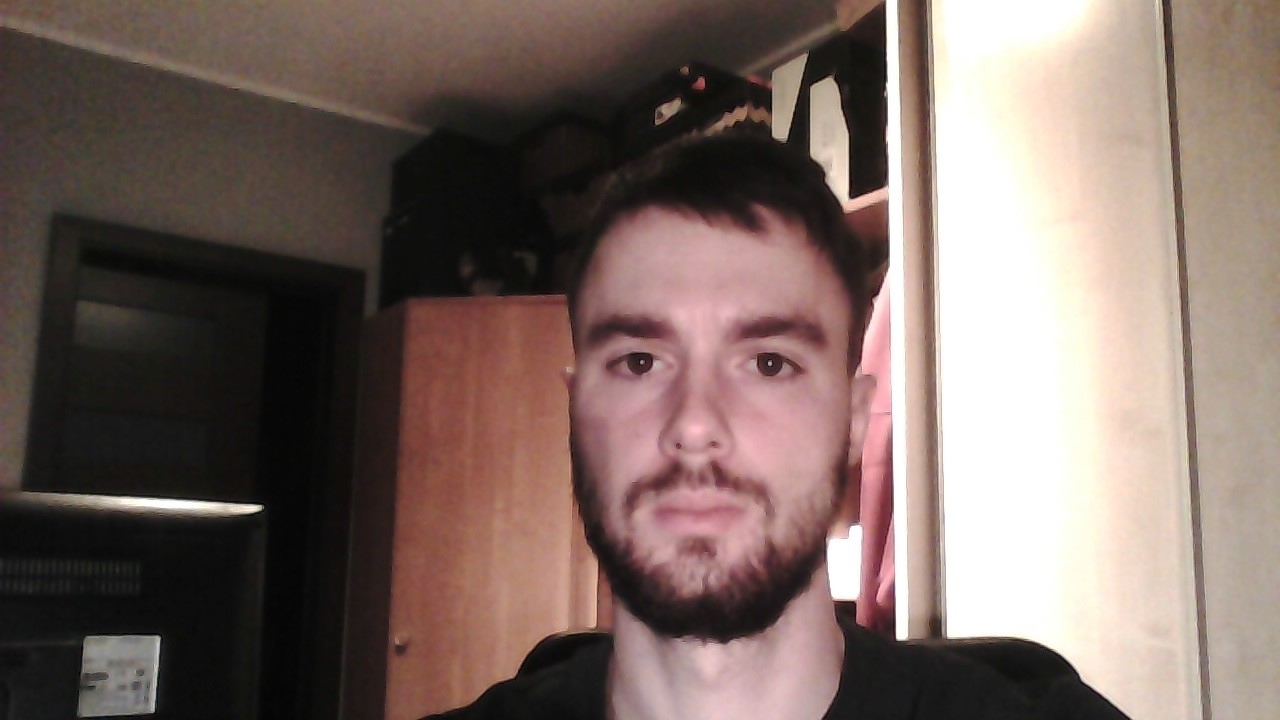
\includegraphics[width=\linewidth, height=20mm]{detekcja/3_input.jpg}
    	\end{minipage}
		& 
		\begin{minipage}{.2\textwidth}
      	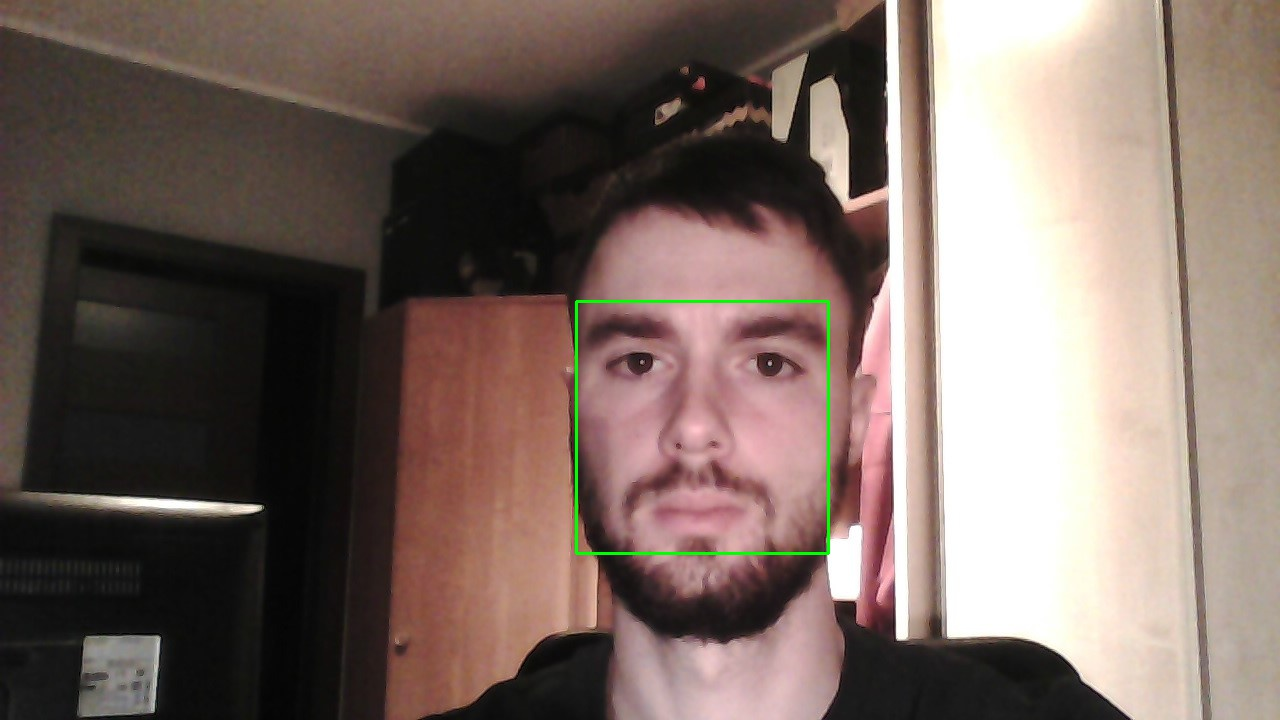
\includegraphics[width=\linewidth, height=20mm]{detekcja/3_haar.jpg}
    	\end{minipage}
		& 
		\begin{minipage}{.2\textwidth}
      	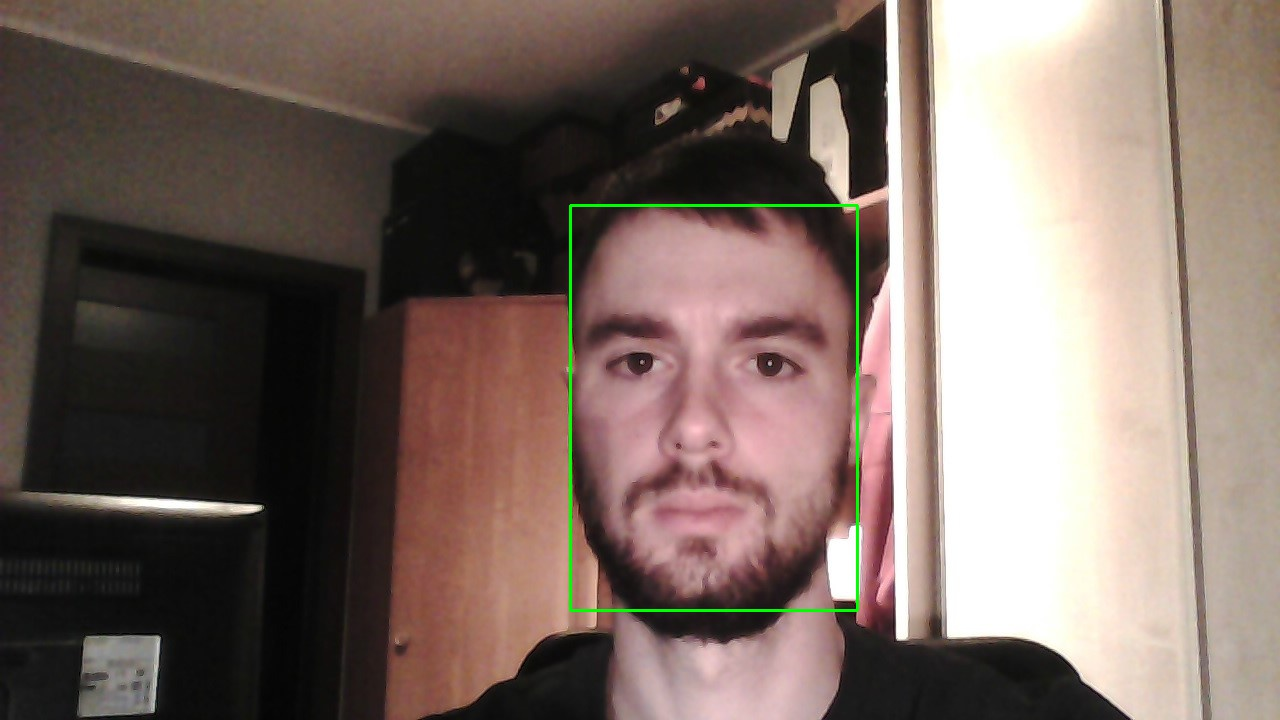
\includegraphics[width=\linewidth, height=20mm]{detekcja/3_dnn.jpg}
    	\end{minipage}
		& 
		\begin{minipage}{.2\textwidth}
      	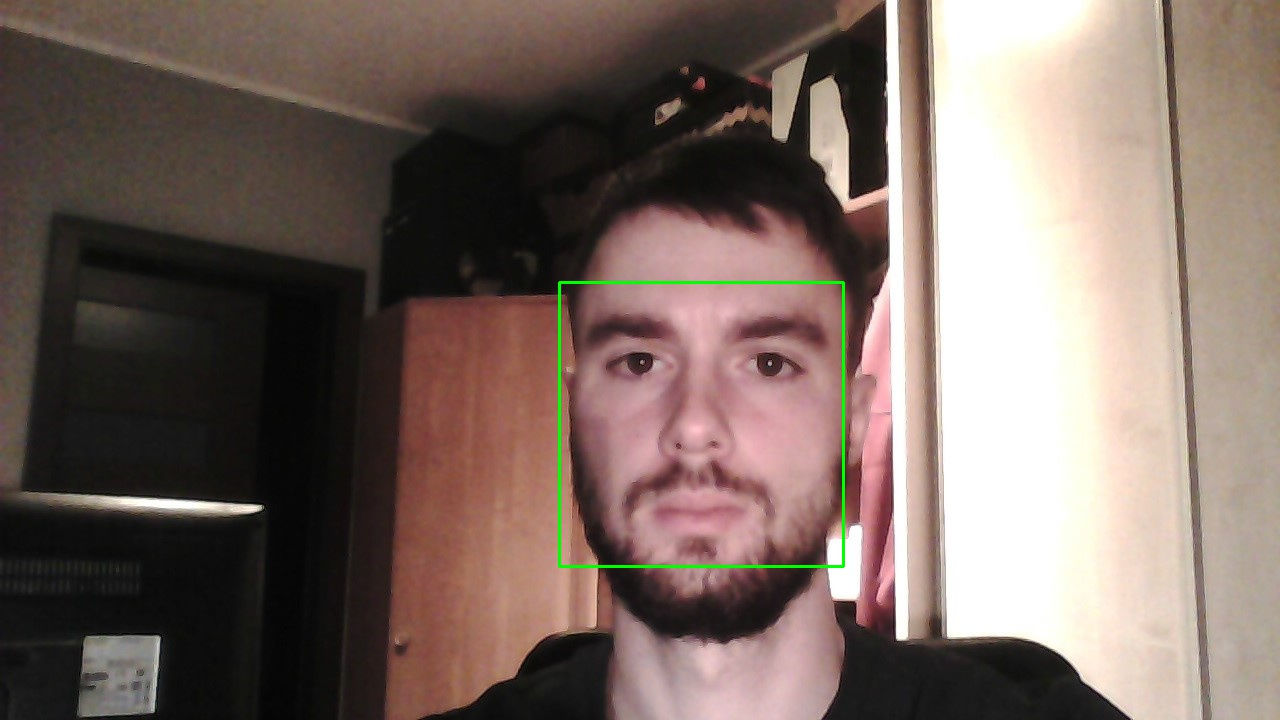
\includegraphics[width=\linewidth, height=20mm]{detekcja/3_azure.jpg}
    	\end{minipage}	
		\\
  		\hline
  		2&		\begin{minipage}{.2\textwidth}
      	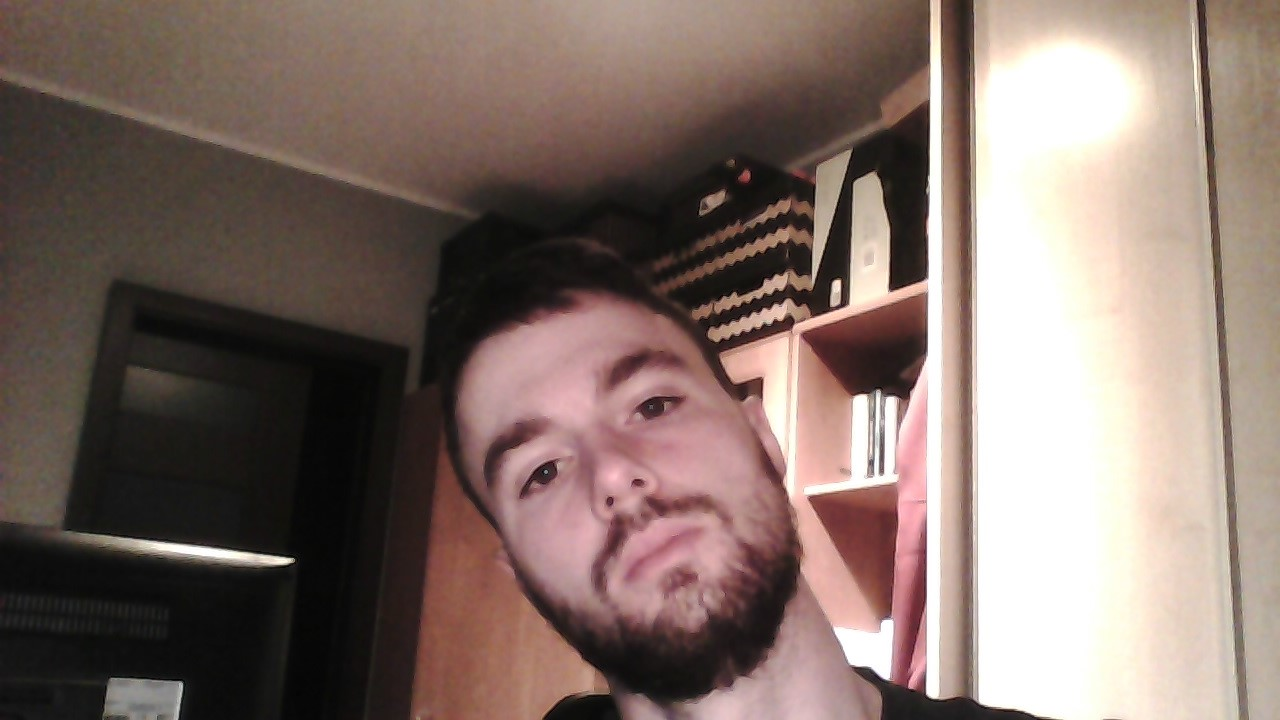
\includegraphics[width=\linewidth, height=20mm]{detekcja/4_input.jpg}
    	\end{minipage}
		& 
		\begin{minipage}{.2\textwidth}
      	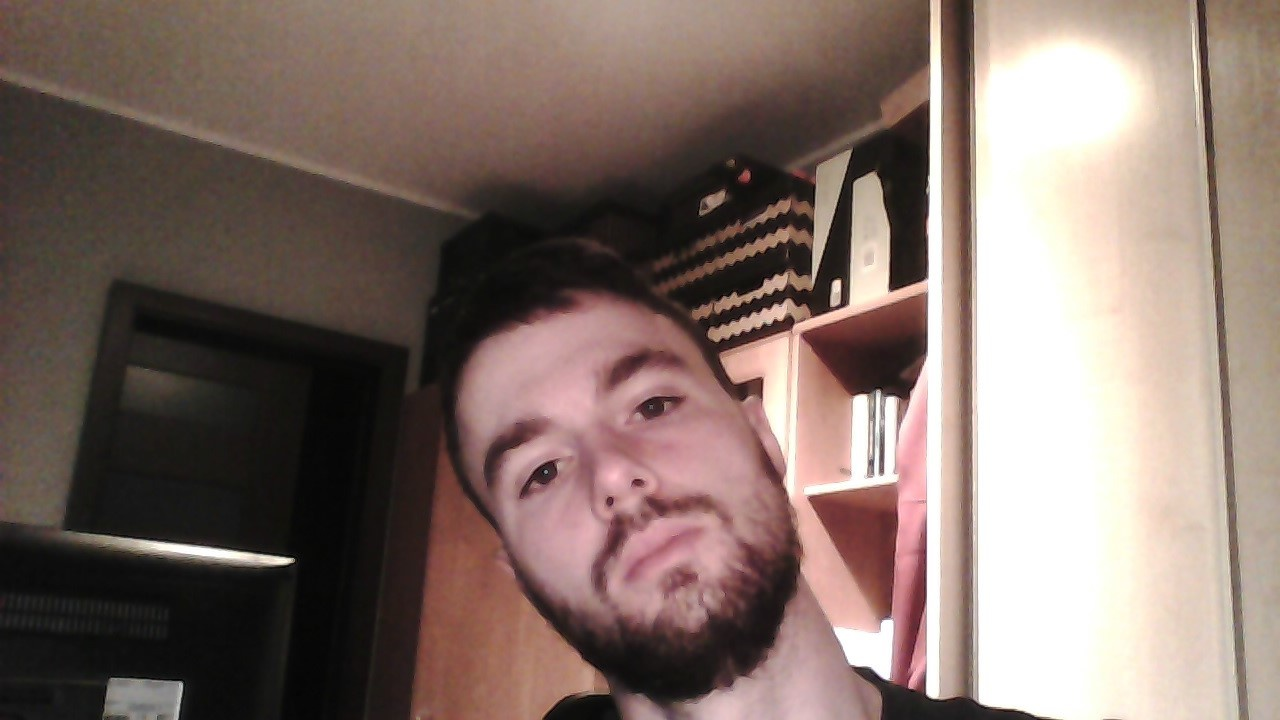
\includegraphics[width=\linewidth, height=20mm]{detekcja/4_haar.jpg}
    	\end{minipage}
		& 
		\begin{minipage}{.2\textwidth}
      	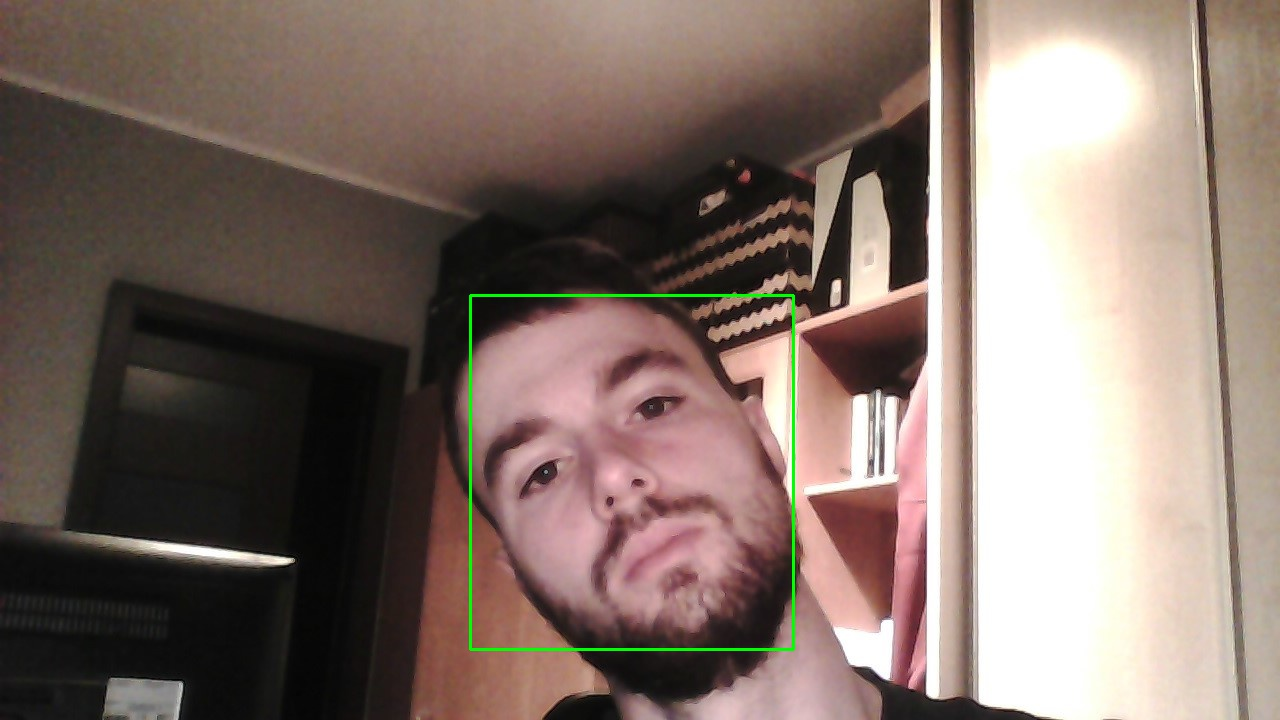
\includegraphics[width=\linewidth, height=20mm]{detekcja/4_dnn.jpg}
    	\end{minipage}
		& 
		\begin{minipage}{.2\textwidth}
      	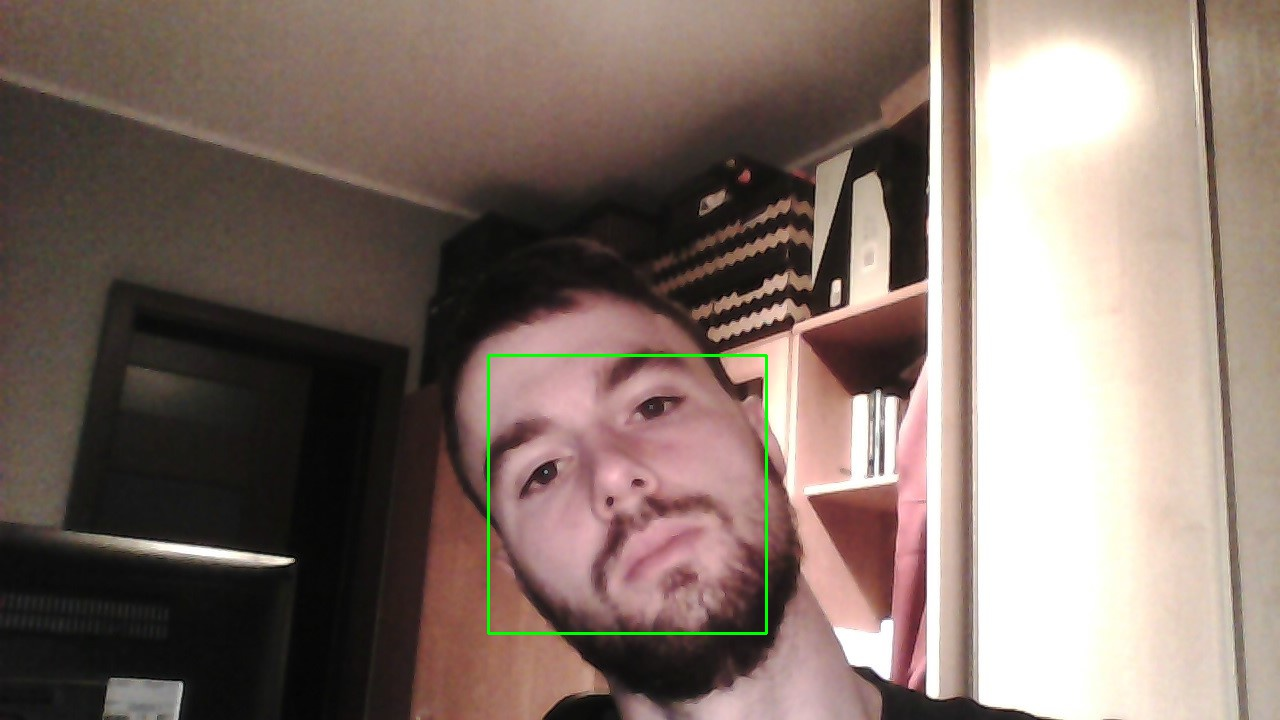
\includegraphics[width=\linewidth, height=20mm]{detekcja/4_azure.jpg}
    	\end{minipage}	
		\\
  		\hline
  		3& 		\begin{minipage}{.2\textwidth}
      	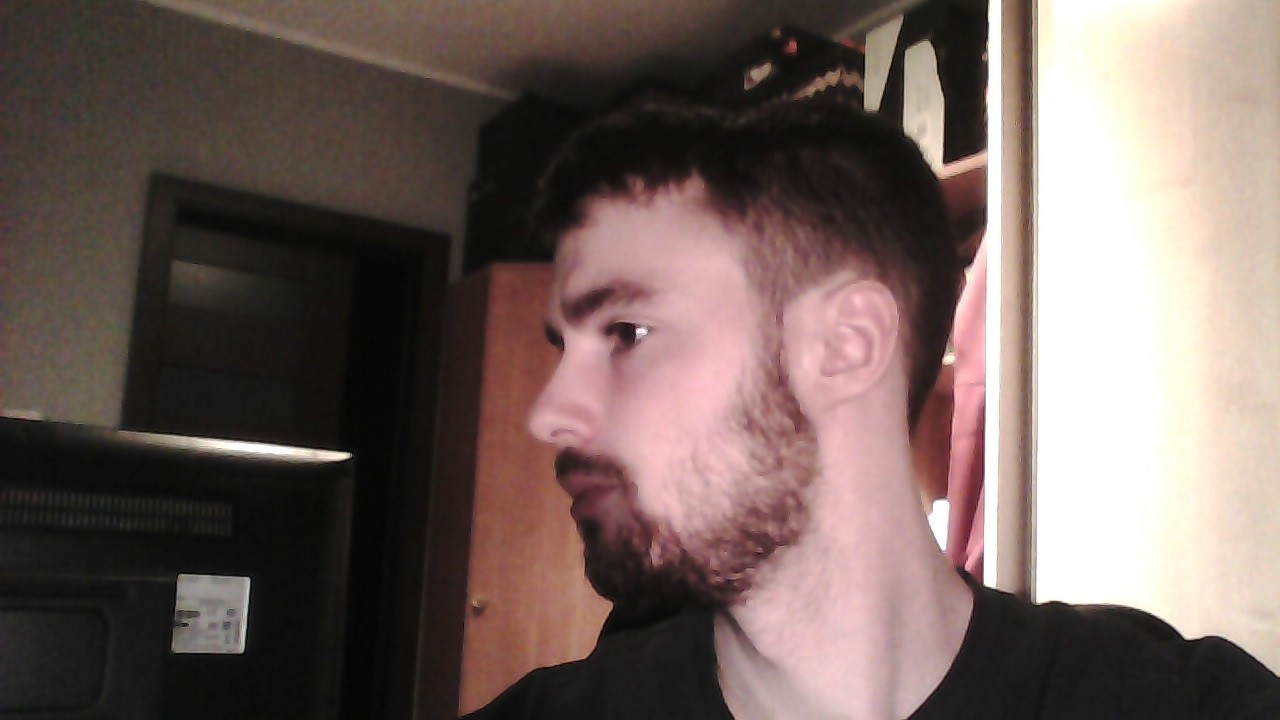
\includegraphics[width=\linewidth, height=20mm]{detekcja/5_input.jpg}
    	\end{minipage}
		& 
		\begin{minipage}{.2\textwidth}
      	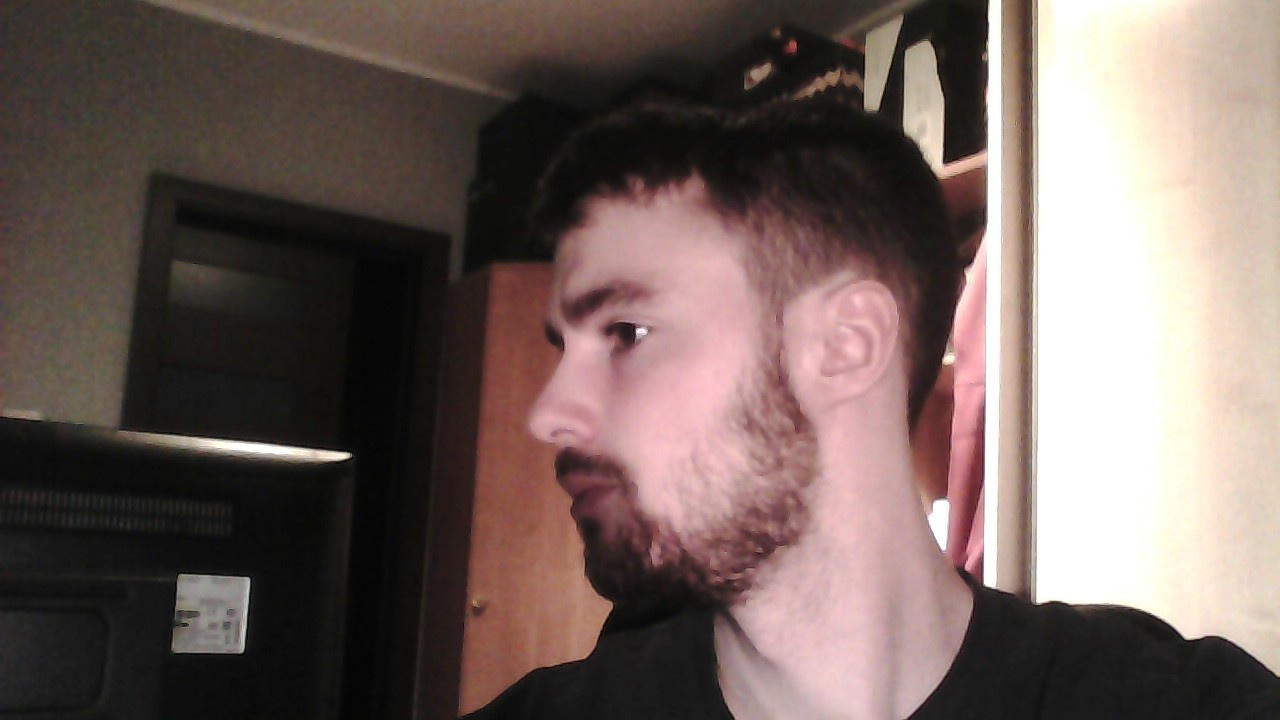
\includegraphics[width=\linewidth, height=20mm]{detekcja/5_haar.jpg}
    	\end{minipage}
		& 
		\begin{minipage}{.2\textwidth}
      	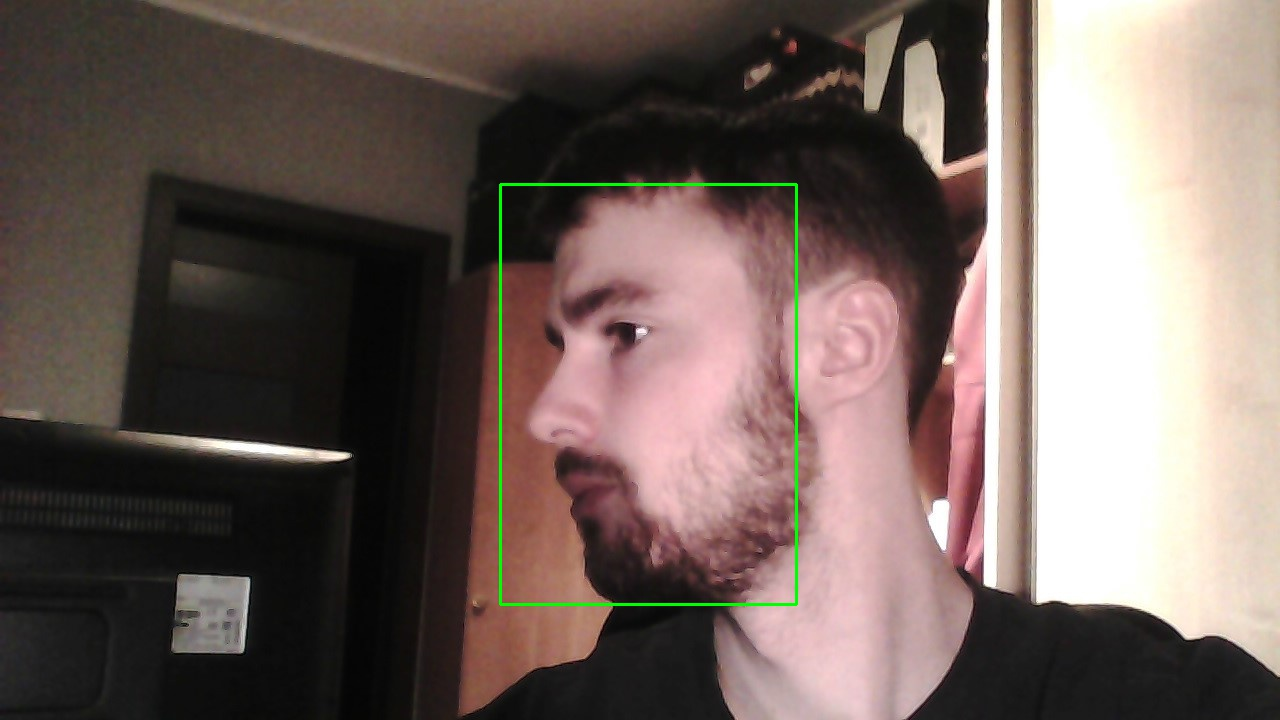
\includegraphics[width=\linewidth, height=20mm]{detekcja/5_dnn.jpg}
    	\end{minipage}
		& 
		\begin{minipage}{.2\textwidth}
      	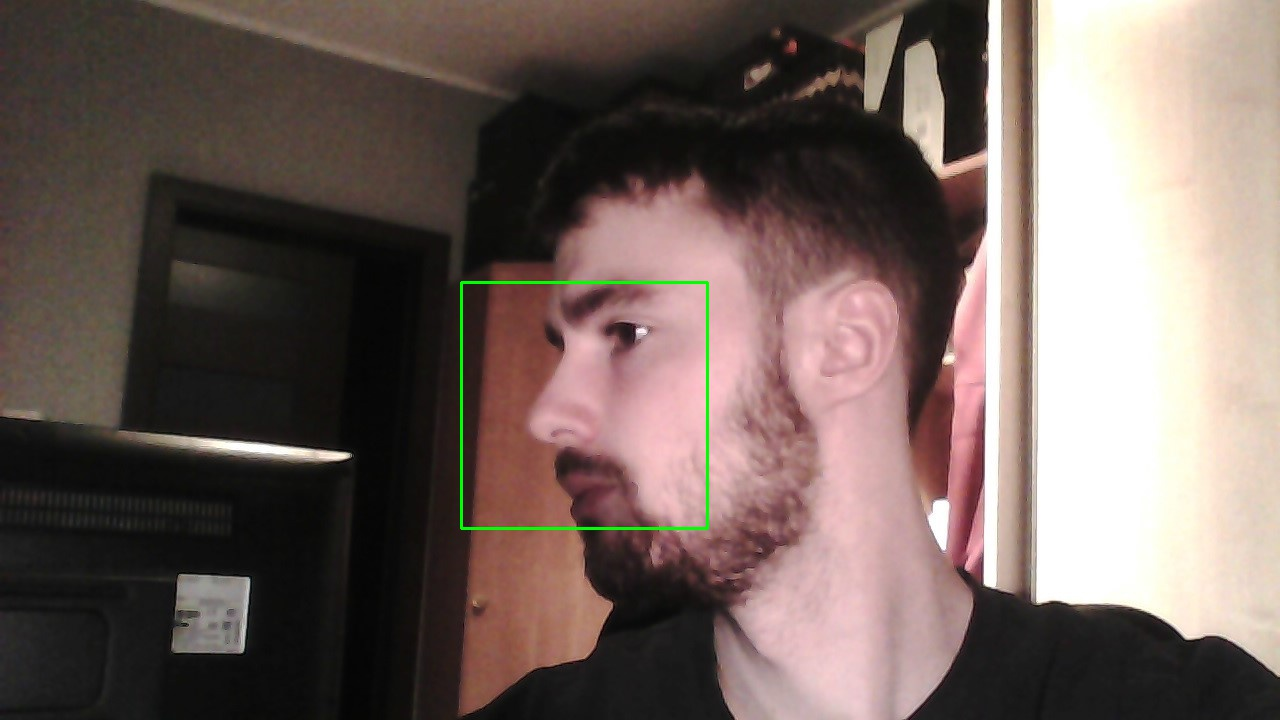
\includegraphics[width=\linewidth, height=20mm]{detekcja/5_azure.jpg}
    	\end{minipage}	
		\\
  		\hline
  		4&  		\begin{minipage}{.2\textwidth}
      	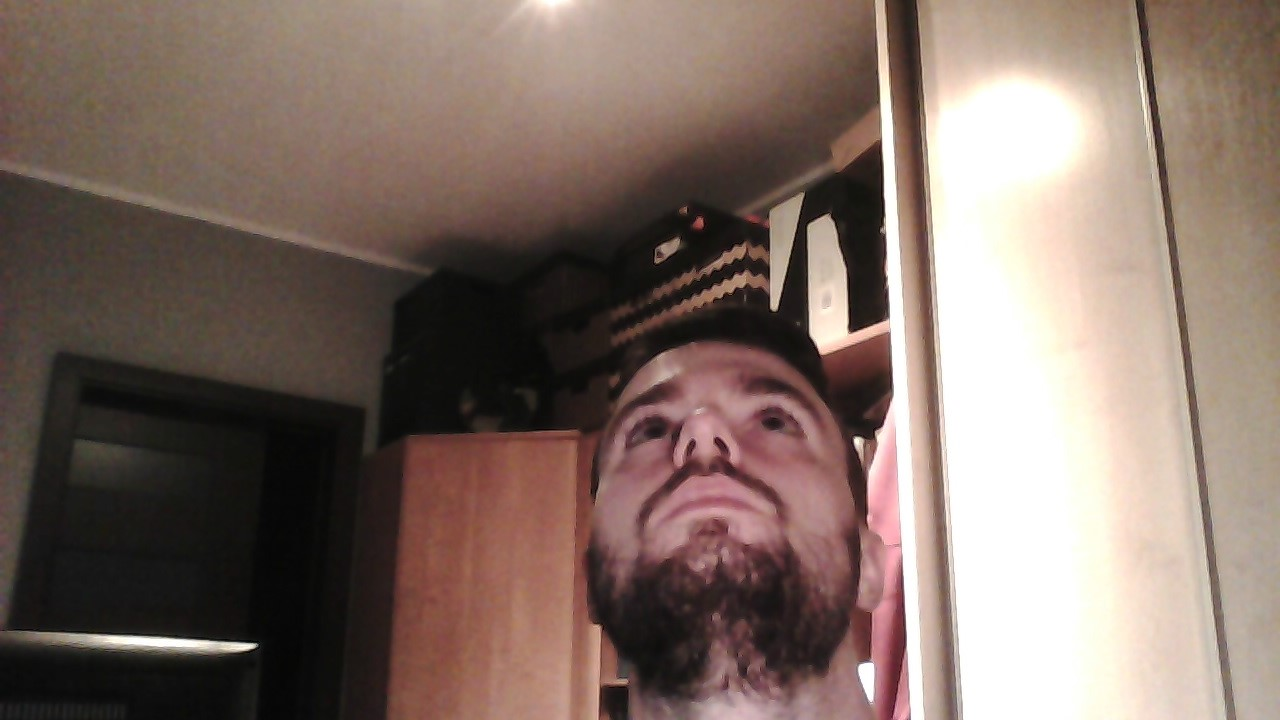
\includegraphics[width=\linewidth, height=20mm]{detekcja/6_input.jpg}
    	\end{minipage}
		& 
		\begin{minipage}{.2\textwidth}
      	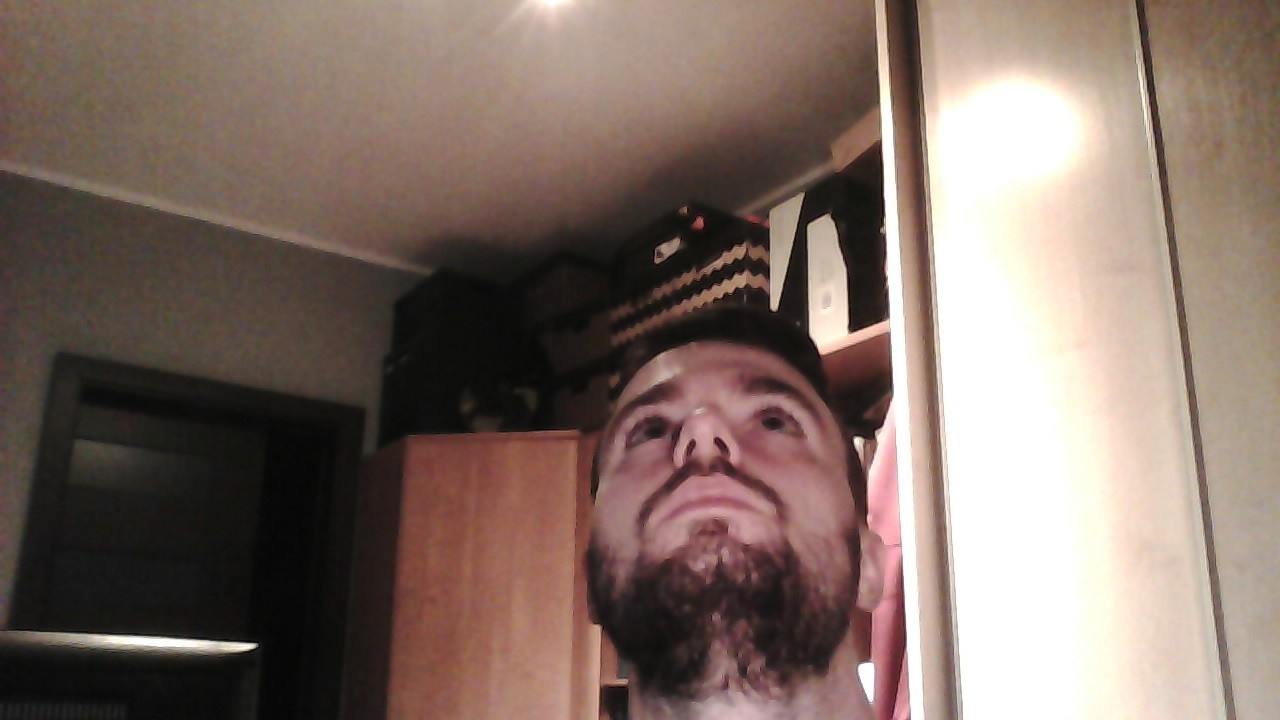
\includegraphics[width=\linewidth, height=20mm]{detekcja/6_haar.jpg}
    	\end{minipage}
		& 
		\begin{minipage}{.2\textwidth}
      	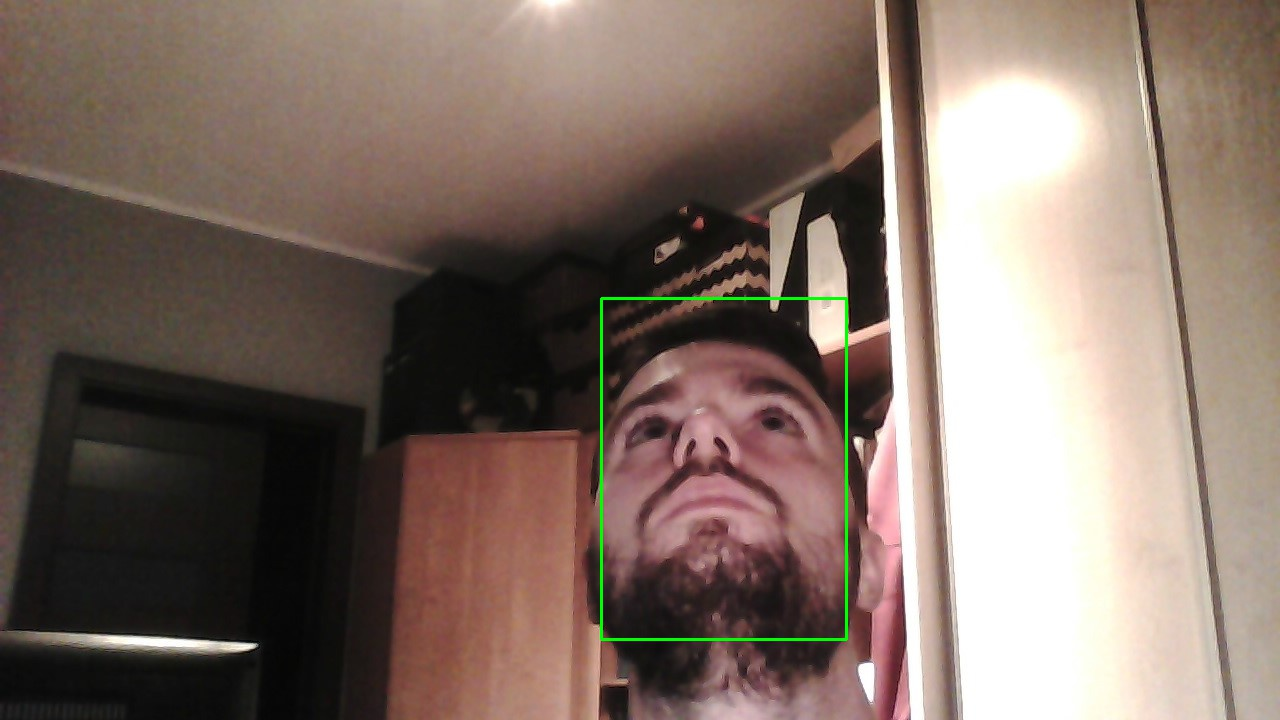
\includegraphics[width=\linewidth, height=20mm]{detekcja/6_dnn.jpg}
    	\end{minipage}
		& 
		\begin{minipage}{.2\textwidth}
      	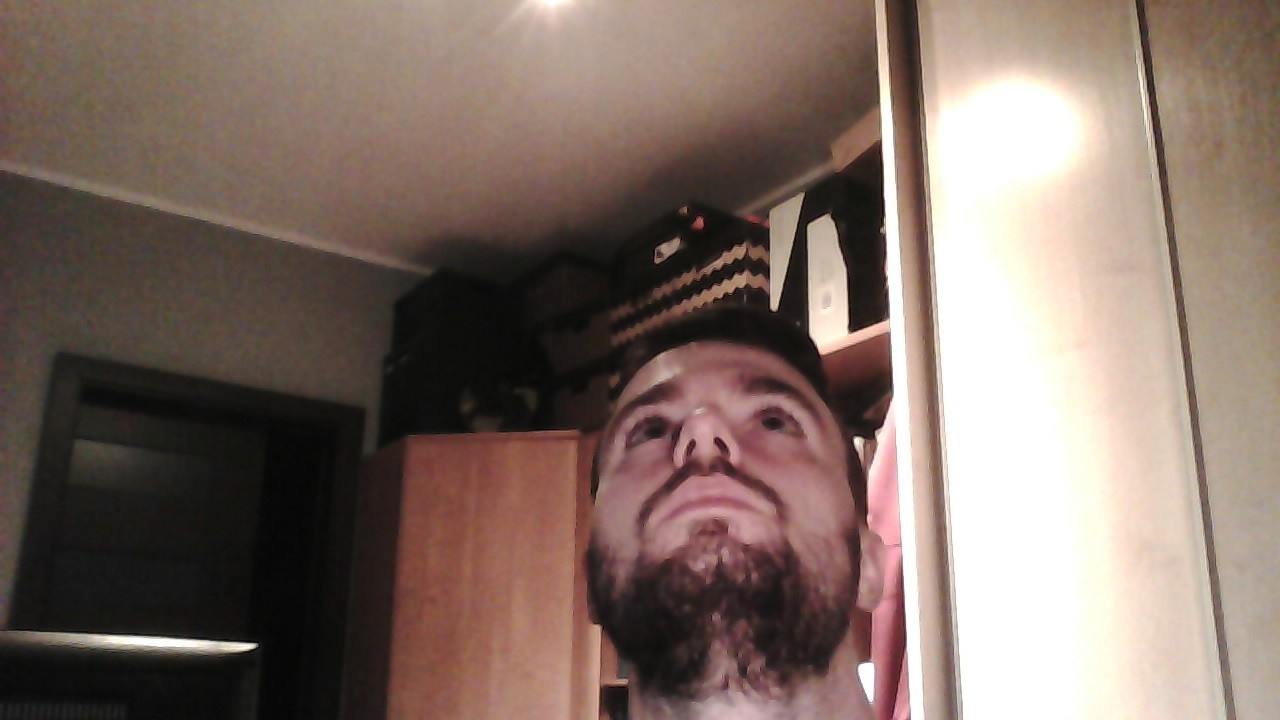
\includegraphics[width=\linewidth, height=20mm]{detekcja/6_azure.jpg}
    	\end{minipage}	
		\\
  		\hline
  		5&  		\begin{minipage}{.2\textwidth}
      	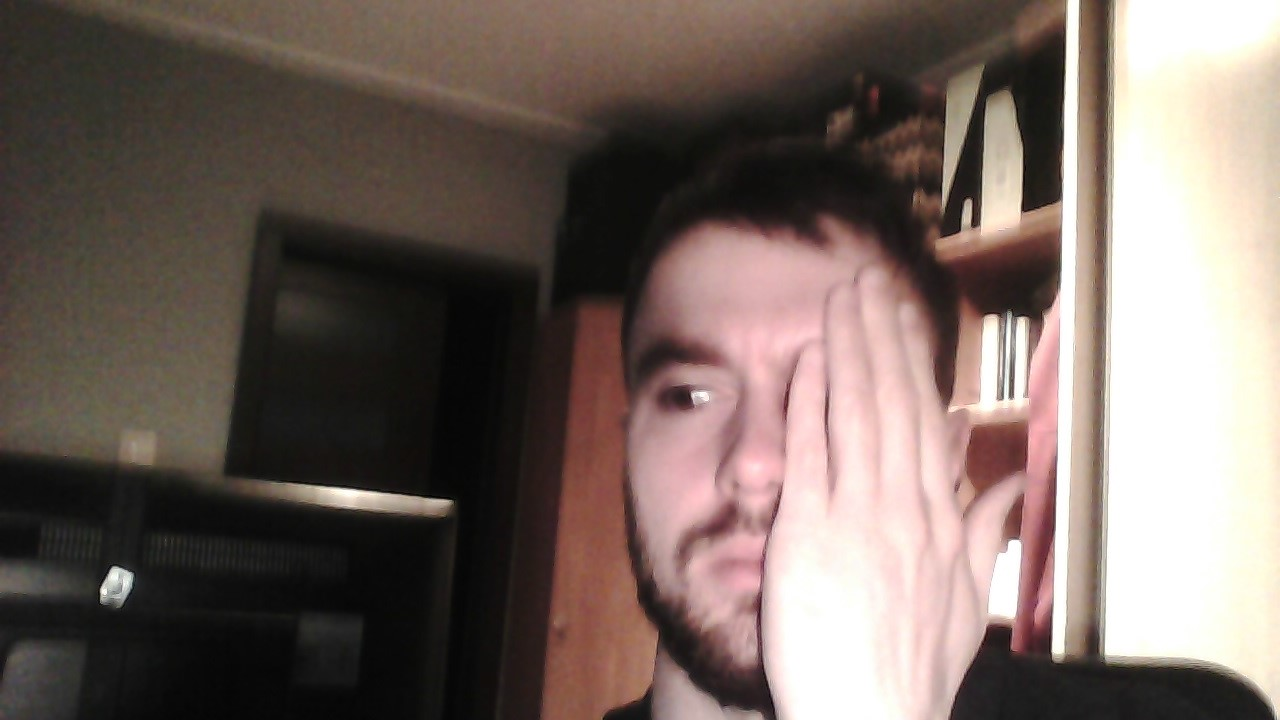
\includegraphics[width=\linewidth, height=20mm]{detekcja/7_input.jpg}
    	\end{minipage}
		& 
		\begin{minipage}{.2\textwidth}
      	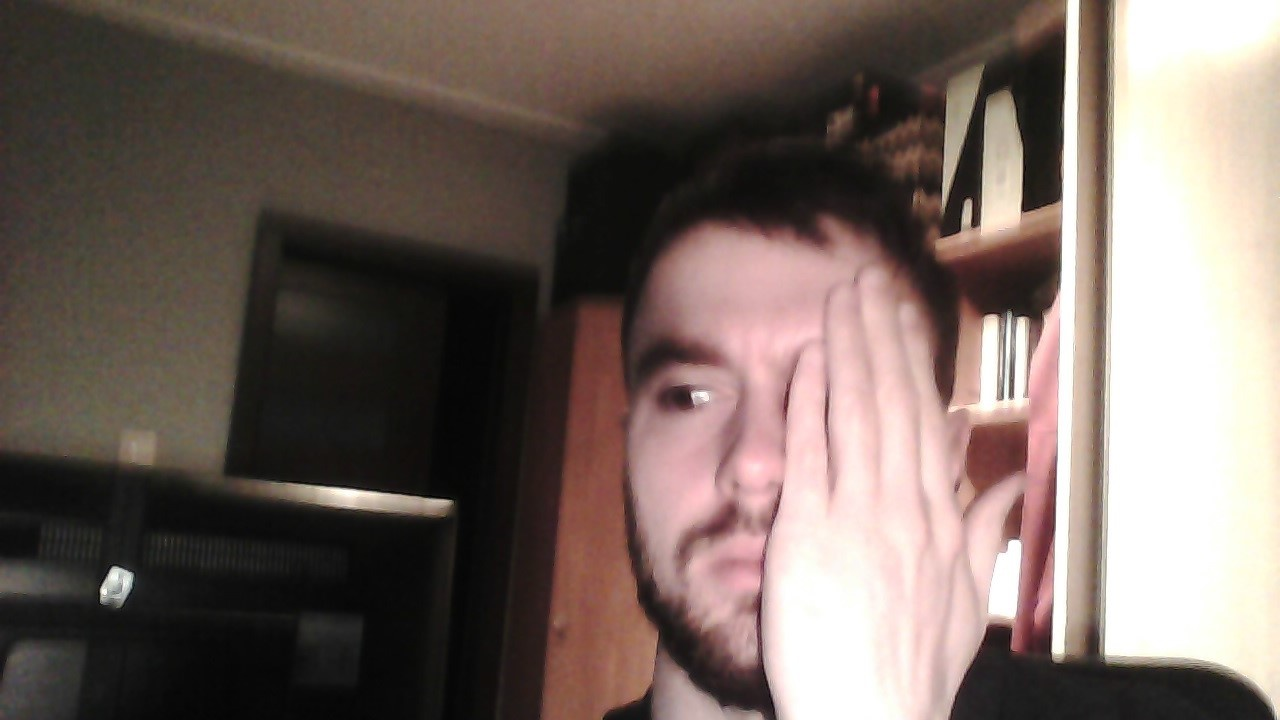
\includegraphics[width=\linewidth, height=20mm]{detekcja/7_haar.jpg}
    	\end{minipage}
		& 
		\begin{minipage}{.2\textwidth}
      	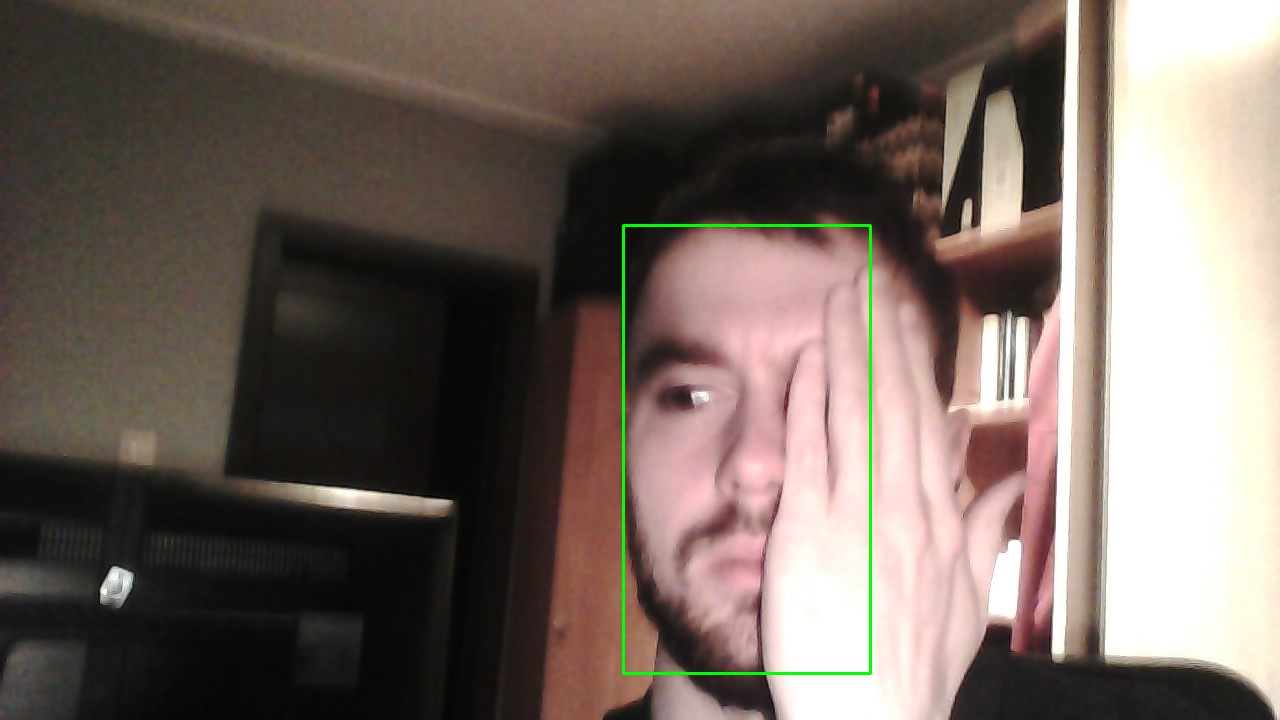
\includegraphics[width=\linewidth, height=20mm]{detekcja/7_dnn.jpg}
    	\end{minipage}
		& 
		\begin{minipage}{.2\textwidth}
      	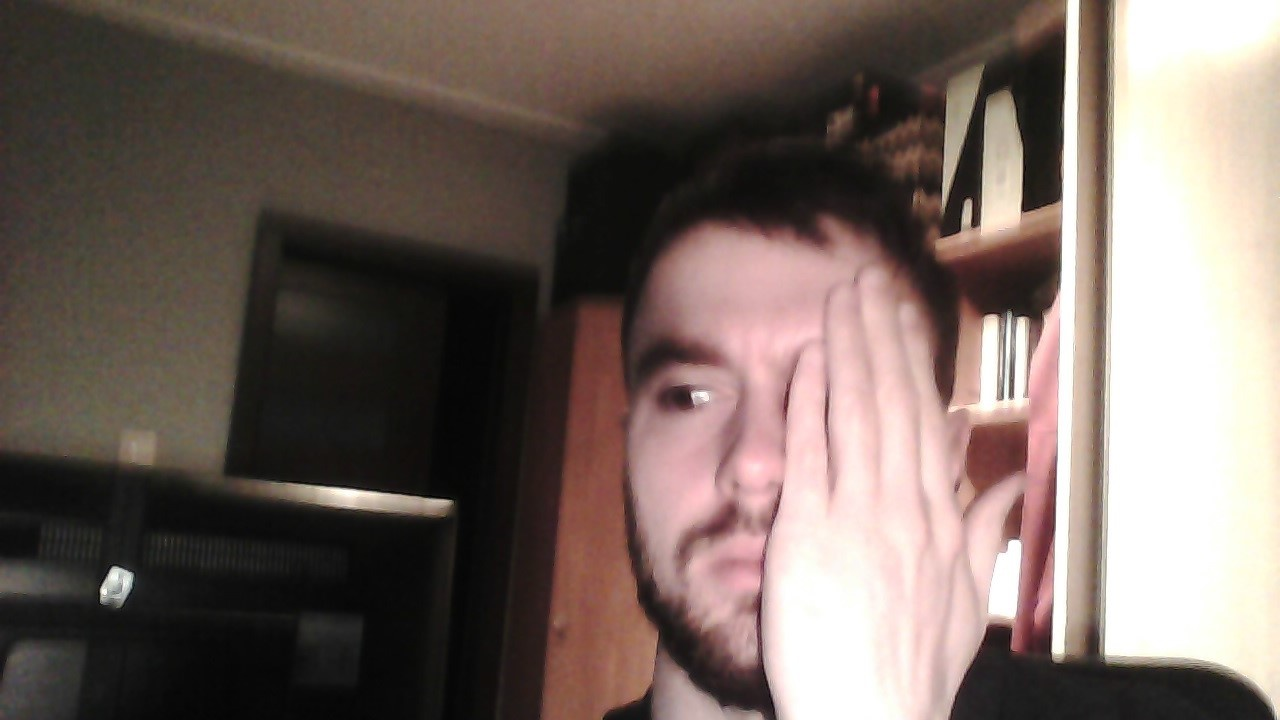
\includegraphics[width=\linewidth, height=20mm]{detekcja/7_azure.jpg}
    	\end{minipage}	
		\\
  		\hline
  		6&  		\begin{minipage}{.2\textwidth}
      	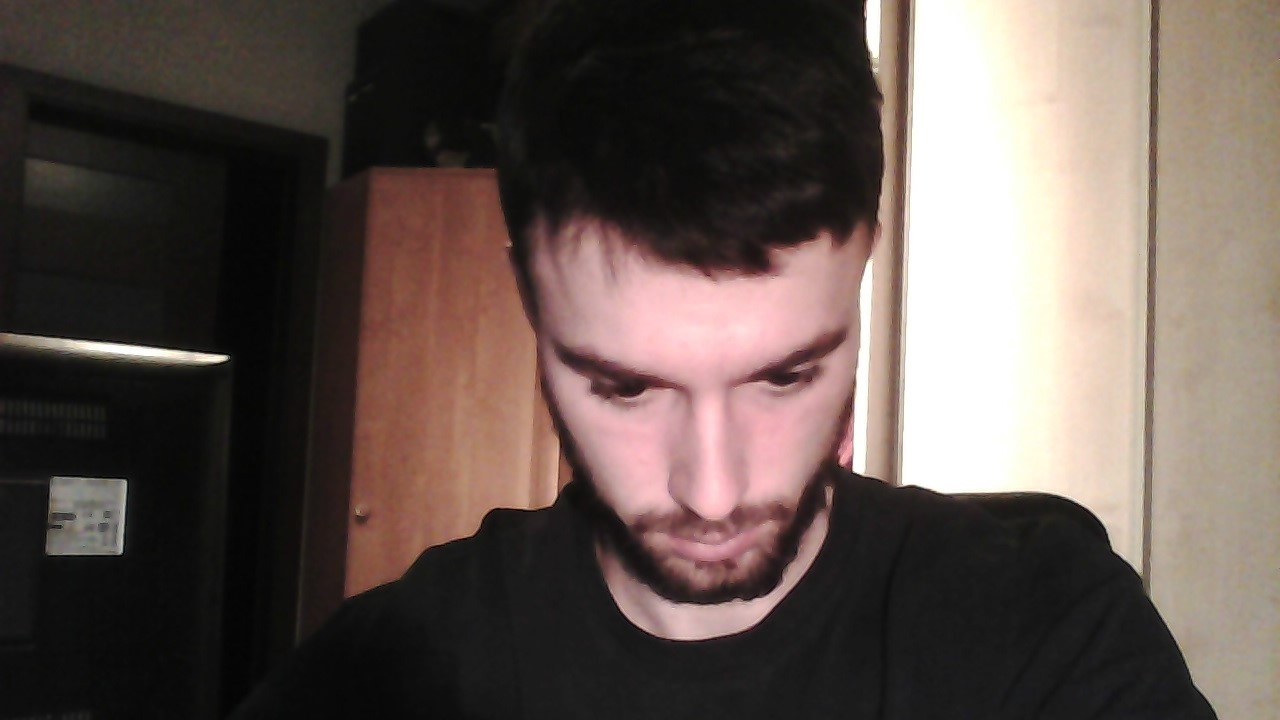
\includegraphics[width=\linewidth, height=20mm]{detekcja/8_input.jpg}
    	\end{minipage}
		& 
		\begin{minipage}{.2\textwidth}
      	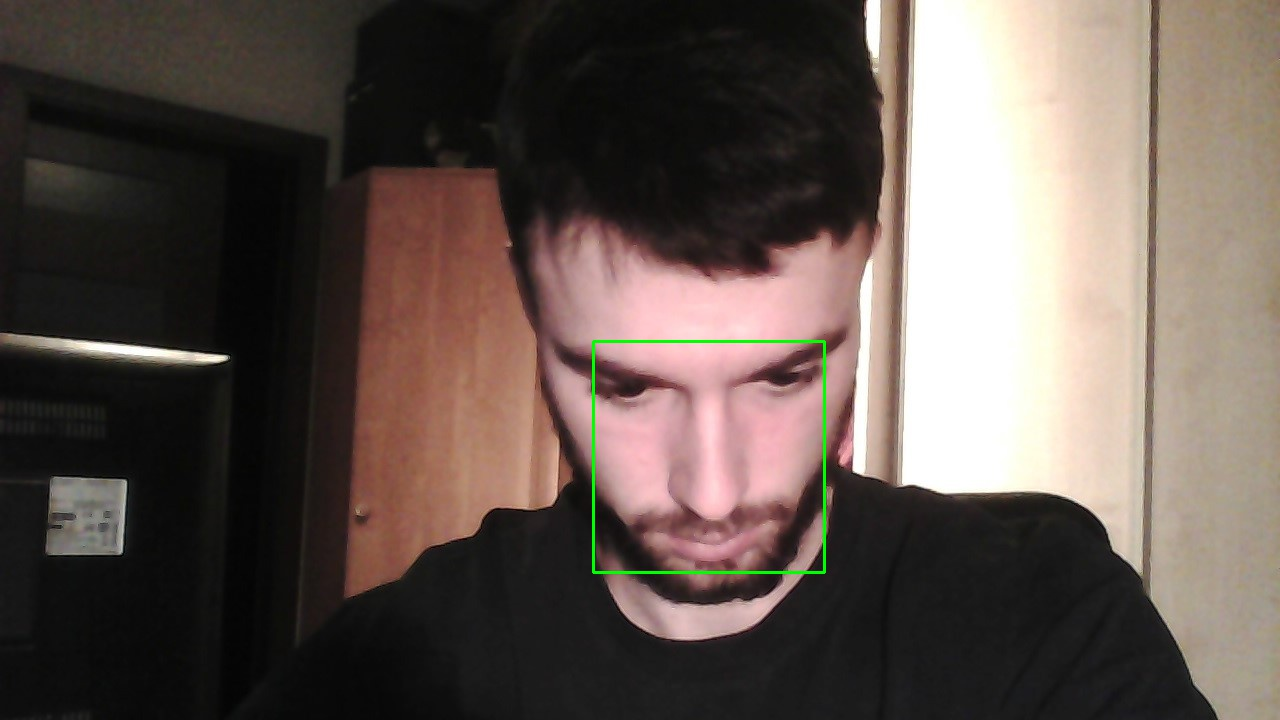
\includegraphics[width=\linewidth, height=20mm]{detekcja/8_haar.jpg}
    	\end{minipage}
		& 
		\begin{minipage}{.2\textwidth}
      	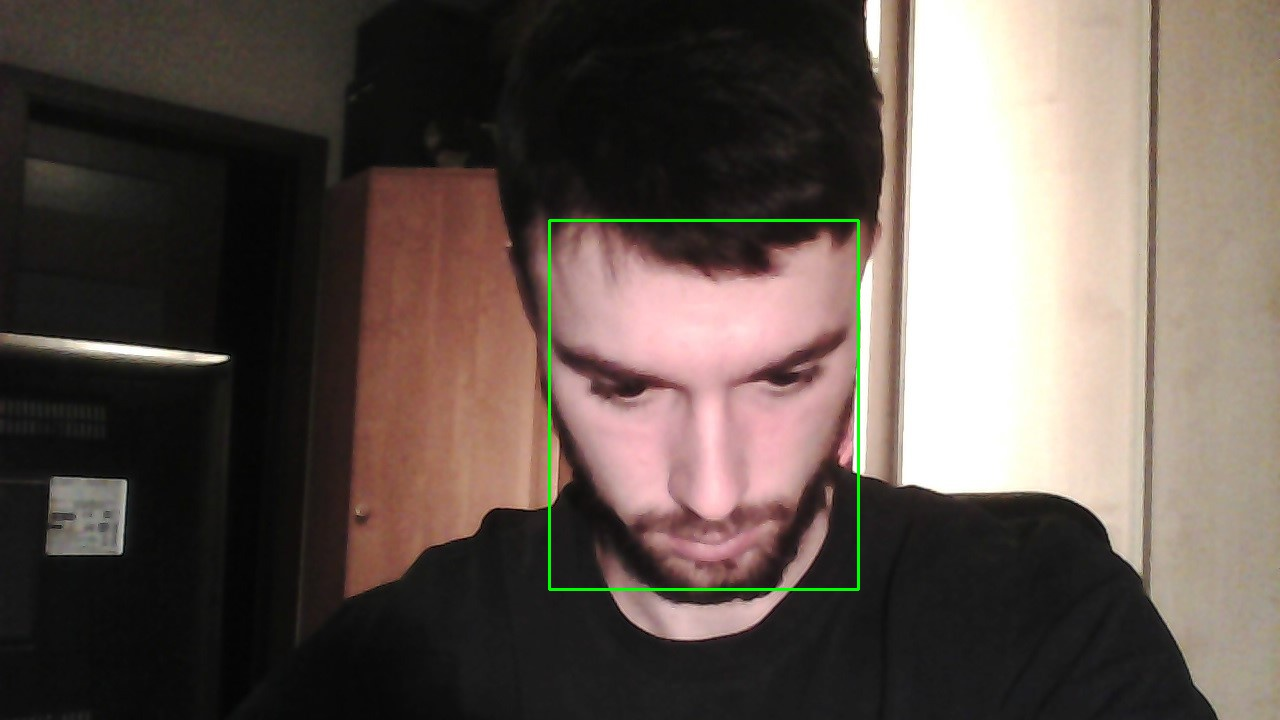
\includegraphics[width=\linewidth, height=20mm]{detekcja/8_dnn.jpg}
    	\end{minipage}
		& 
		\begin{minipage}{.2\textwidth}
      	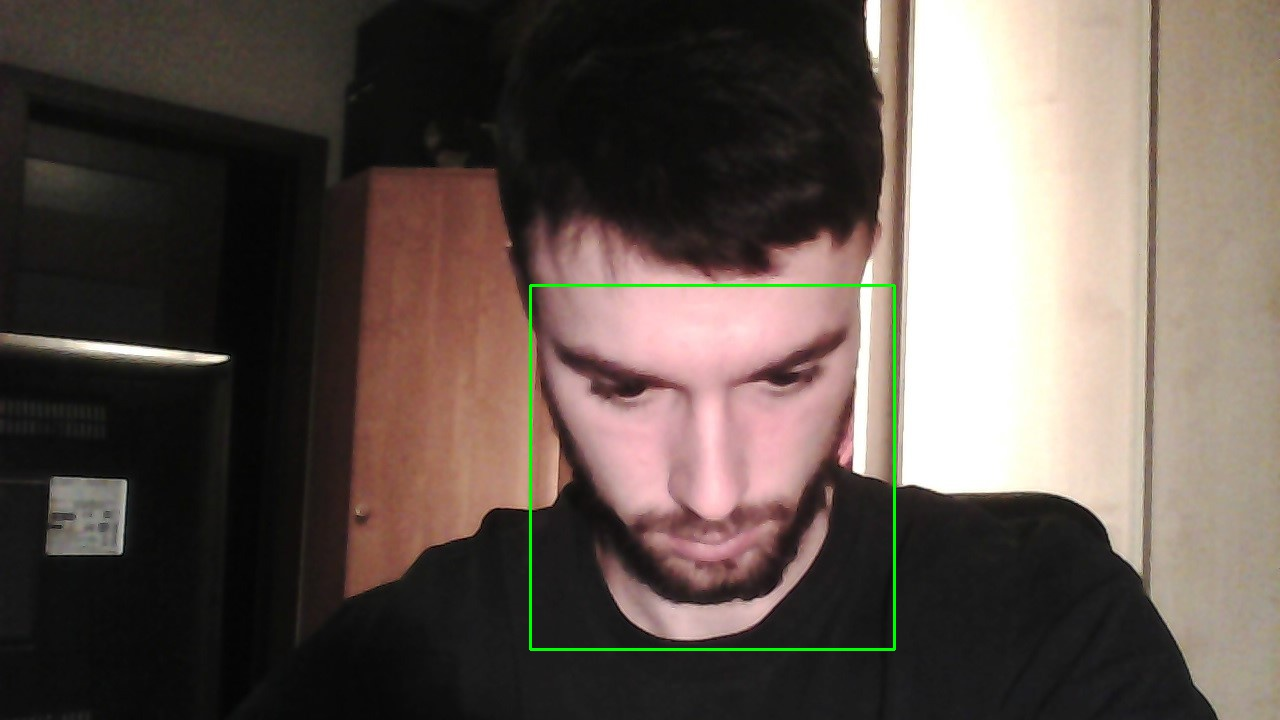
\includegraphics[width=\linewidth, height=20mm]{detekcja/8_azure.jpg}
    	\end{minipage}	
		\\
  		\hline
  		7&  		\begin{minipage}{.2\textwidth}
      	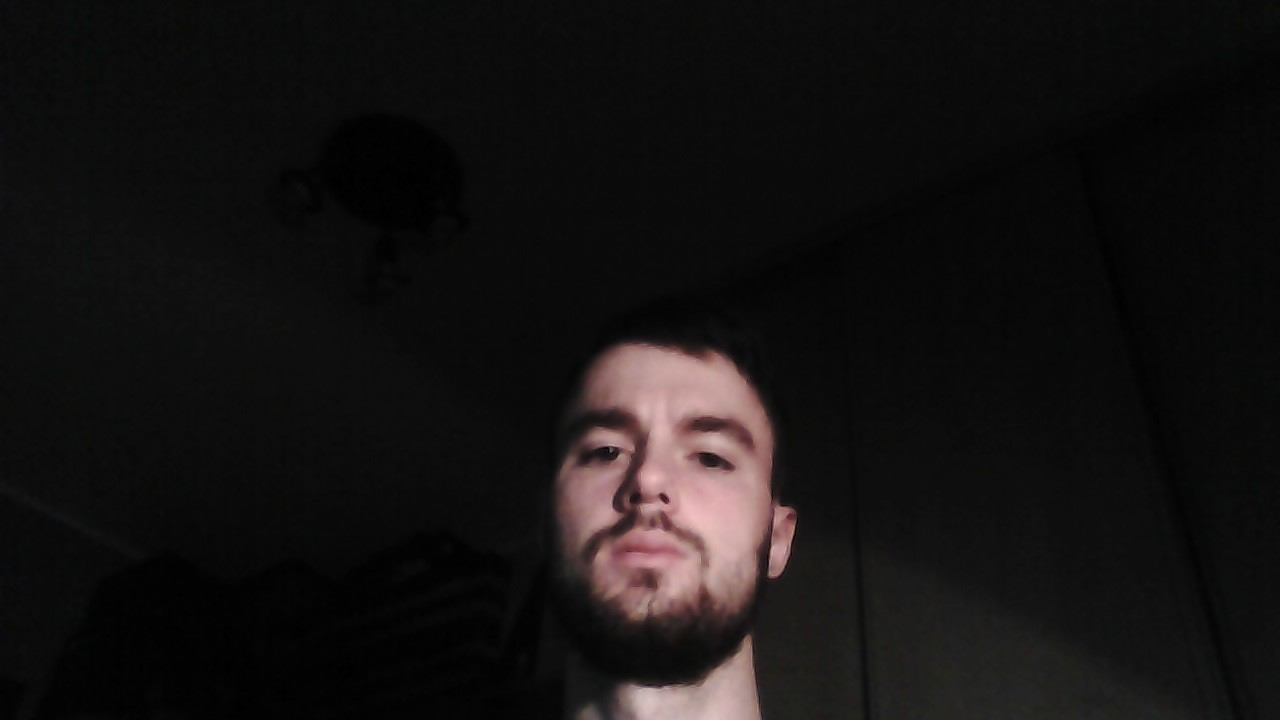
\includegraphics[width=\linewidth, height=20mm]{detekcja/9_input.jpg}
    	\end{minipage}
		& 
		\begin{minipage}{.2\textwidth}
      	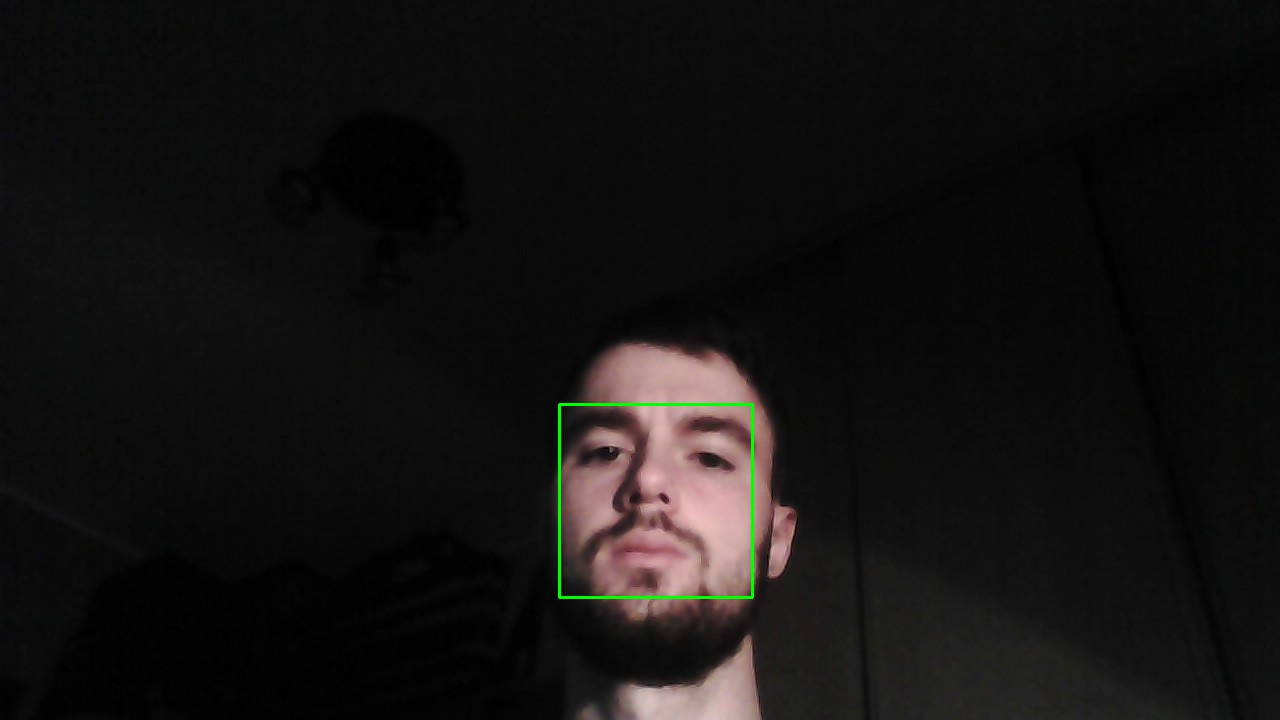
\includegraphics[width=\linewidth, height=20mm]{detekcja/9_haar.jpg}
    	\end{minipage}
		& 
		\begin{minipage}{.2\textwidth}
      	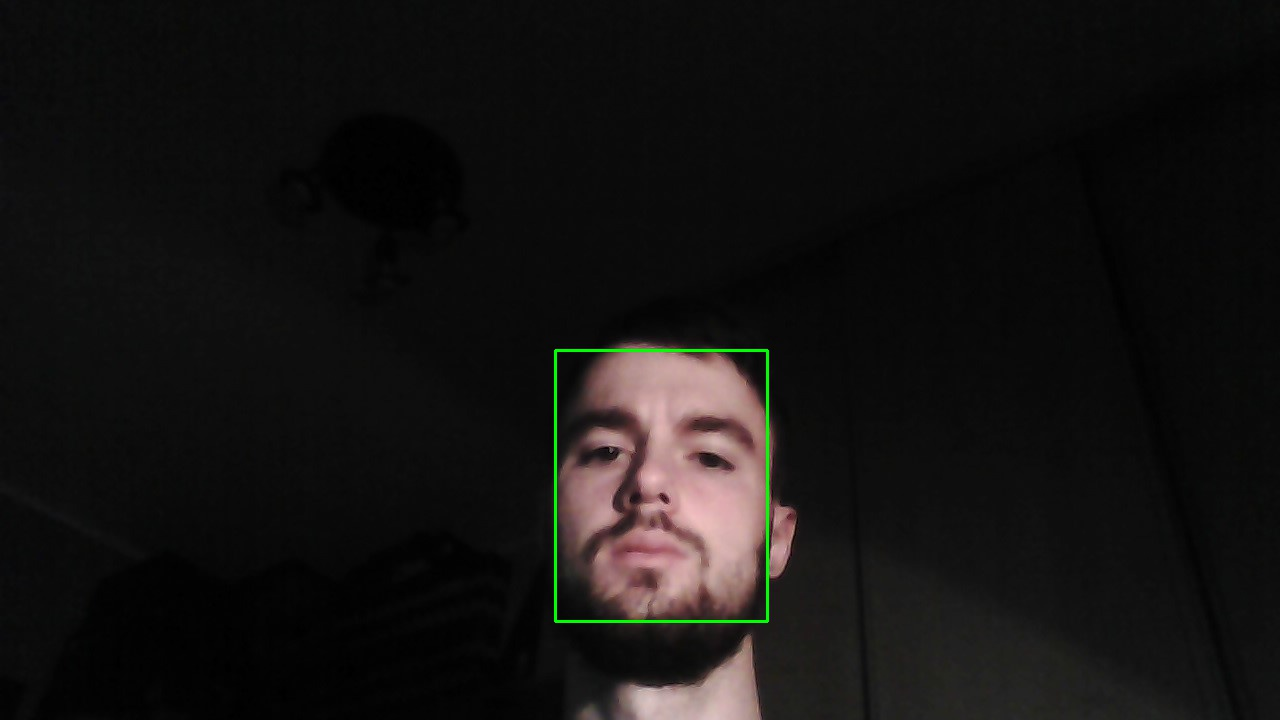
\includegraphics[width=\linewidth, height=20mm]{detekcja/9_dnn.jpg}
    	\end{minipage}
		& 
		\begin{minipage}{.2\textwidth}
      	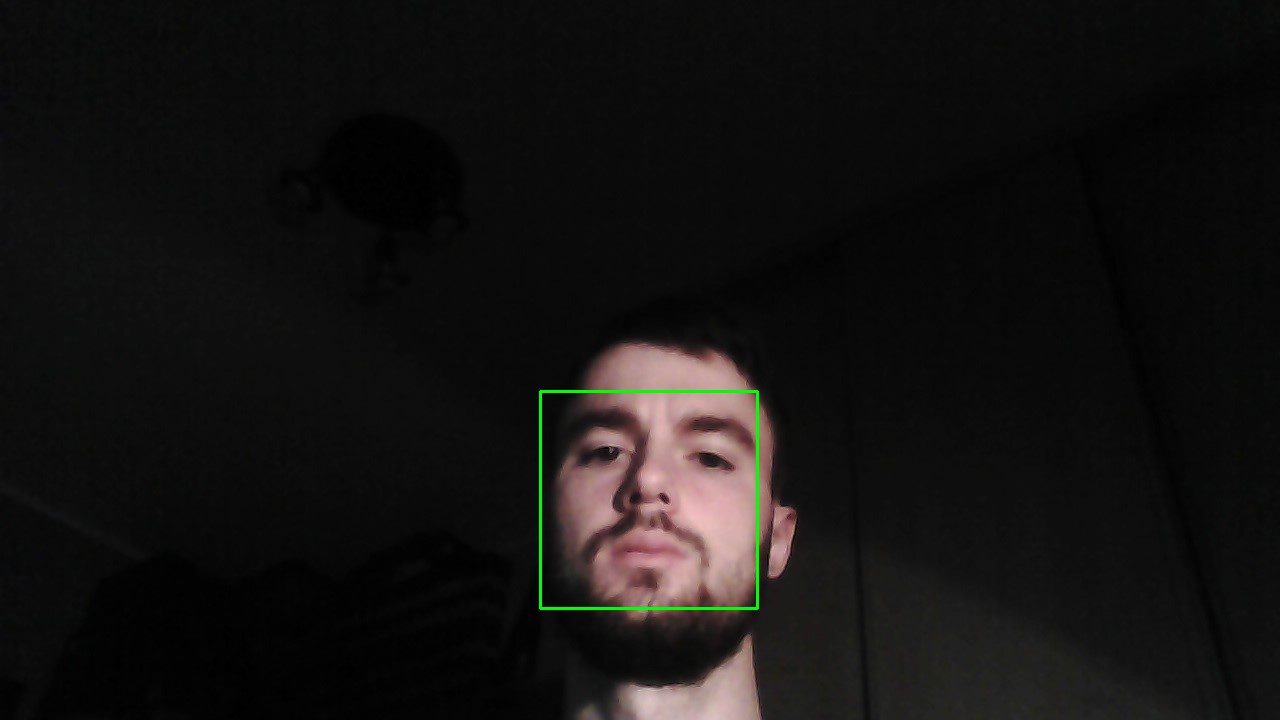
\includegraphics[width=\linewidth, height=20mm]{detekcja/9_azure.jpg}
    	\end{minipage}	
		\\
  		\hline
  		8&  		  		\begin{minipage}{.2\textwidth}
      	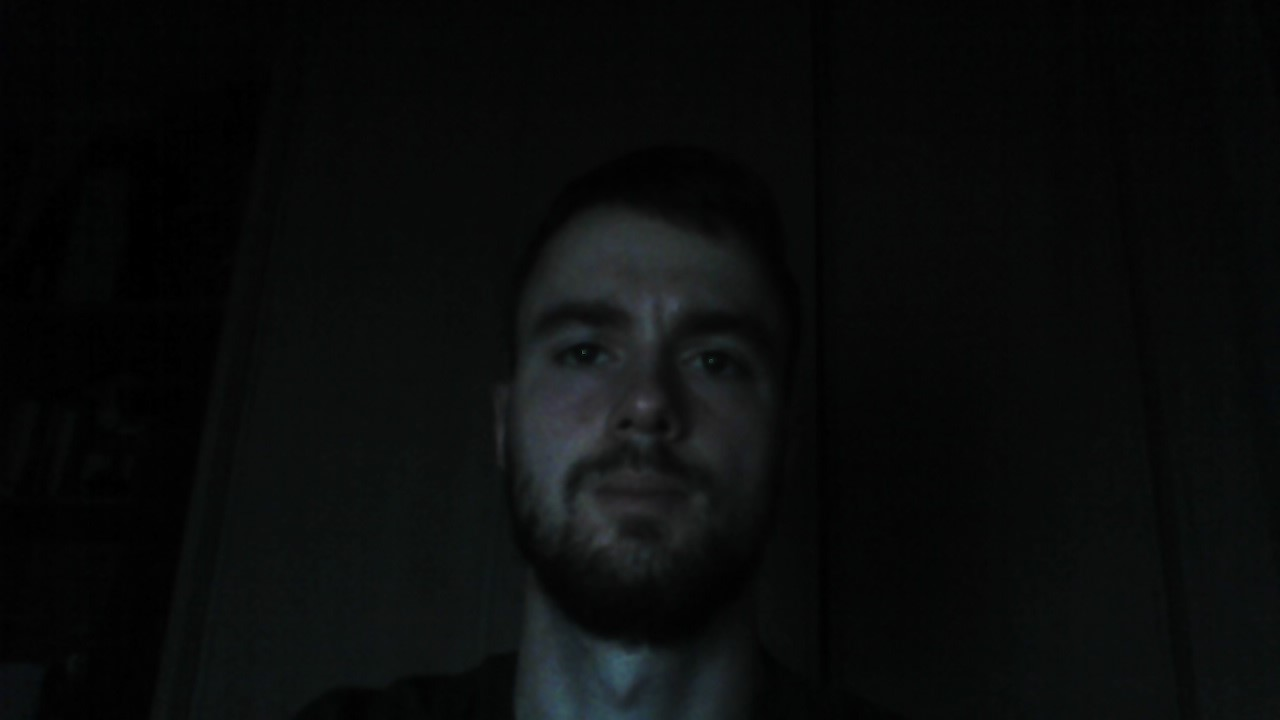
\includegraphics[width=\linewidth, height=20mm]{detekcja/11_input.jpg}
    	\end{minipage}
		& 
		\begin{minipage}{.2\textwidth}
      	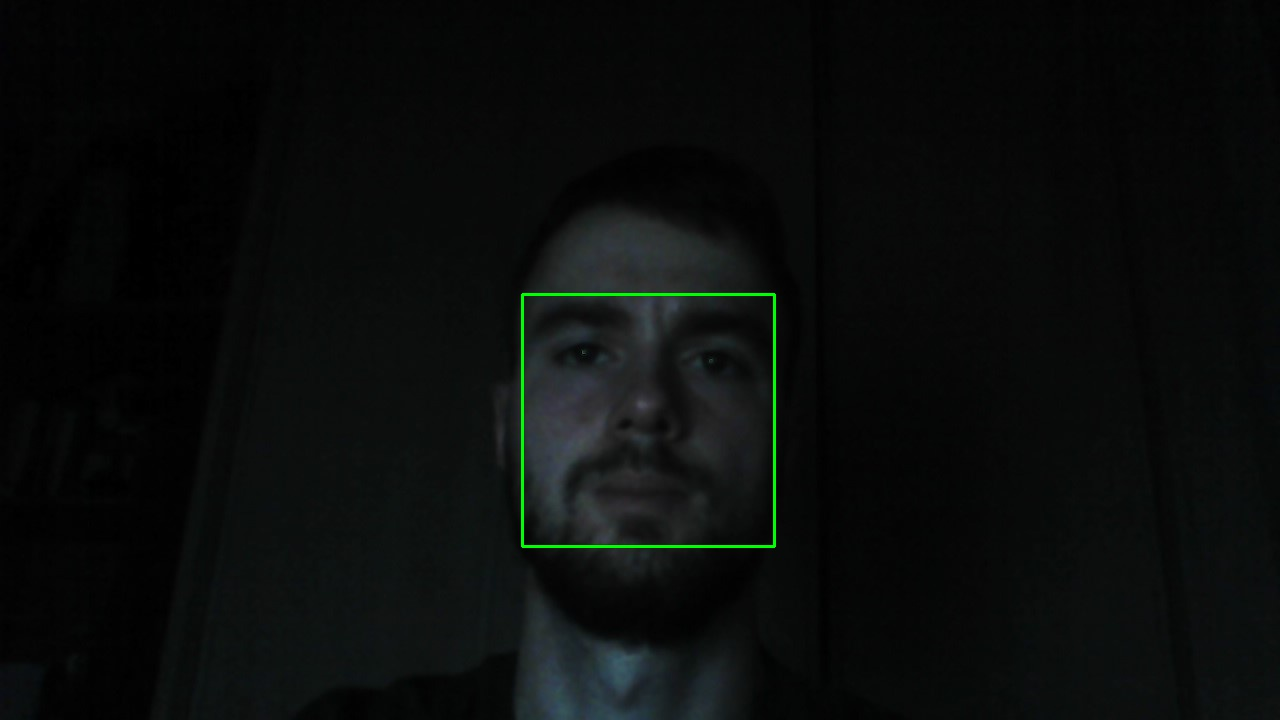
\includegraphics[width=\linewidth, height=20mm]{detekcja/11_haar.jpg}
    	\end{minipage}
		& 
		\begin{minipage}{.2\textwidth}
      	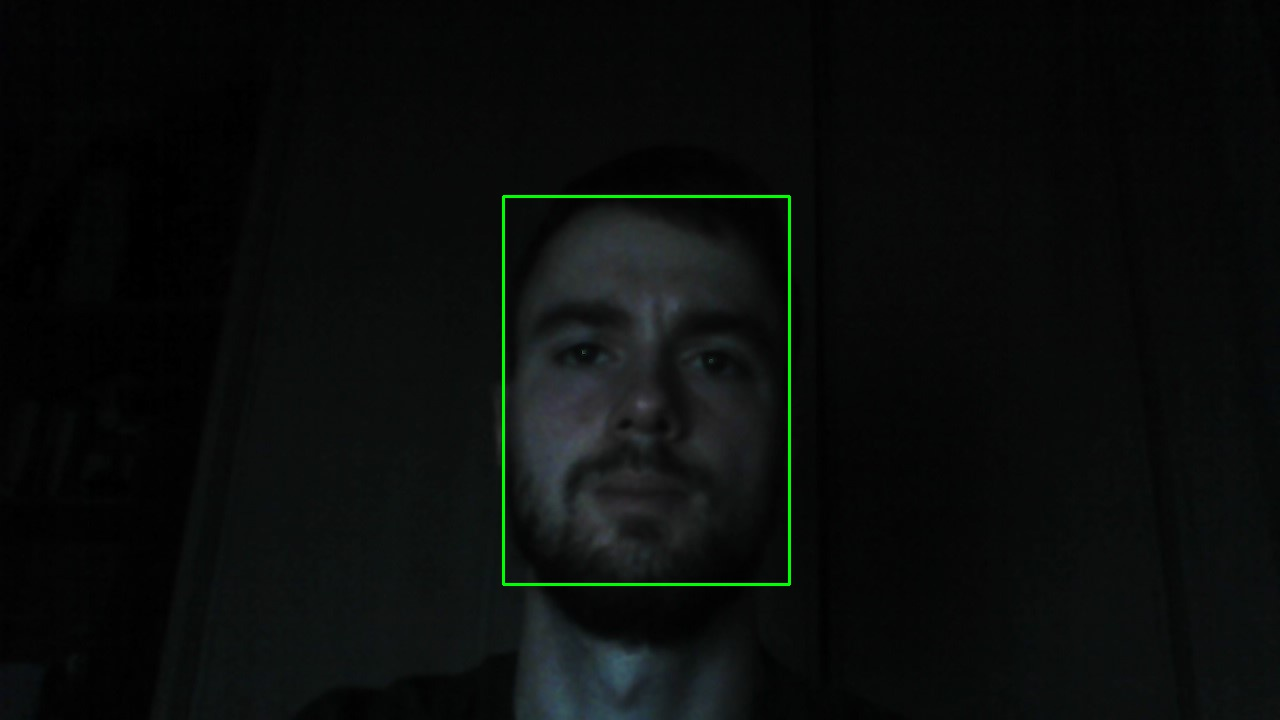
\includegraphics[width=\linewidth, height=20mm]{detekcja/11_dnn.jpg}
    	\end{minipage}
		& 
		\begin{minipage}{.2\textwidth}
      	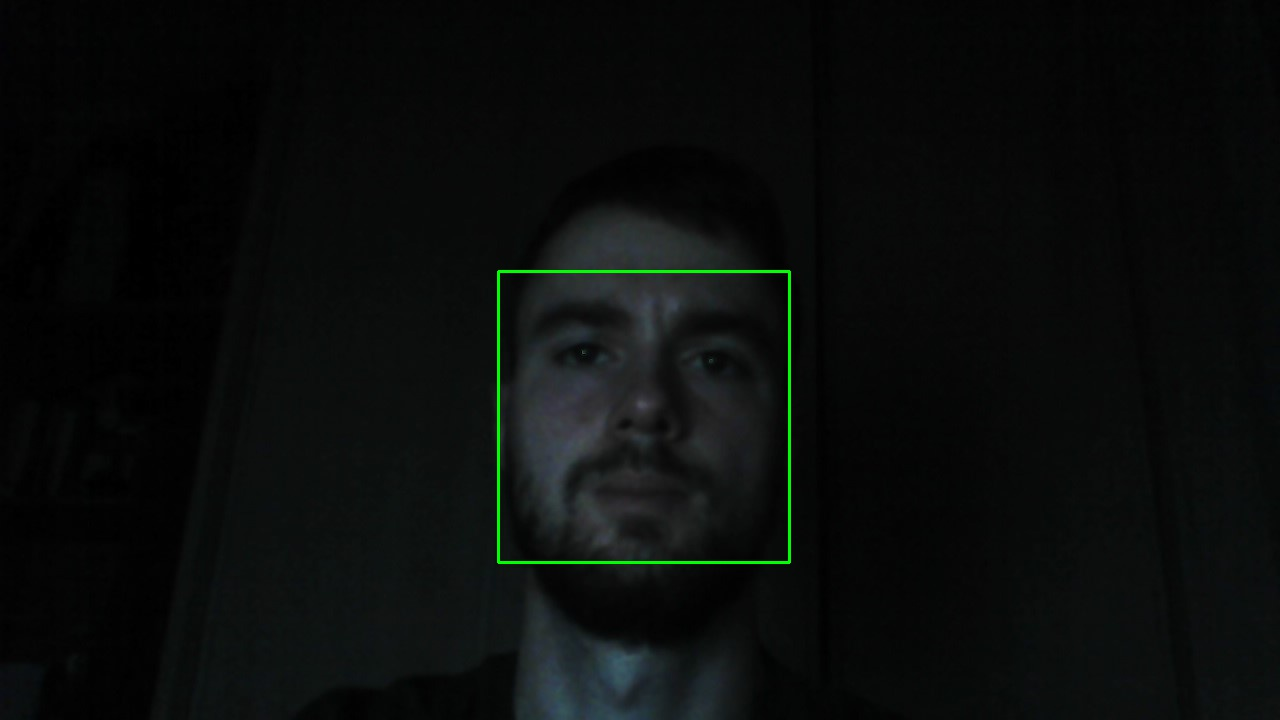
\includegraphics[width=\linewidth, height=20mm]{detekcja/11_azure.jpg}
    	\end{minipage}	
		\\
  		\hline
  		9&  		  		\begin{minipage}{.2\textwidth}
      	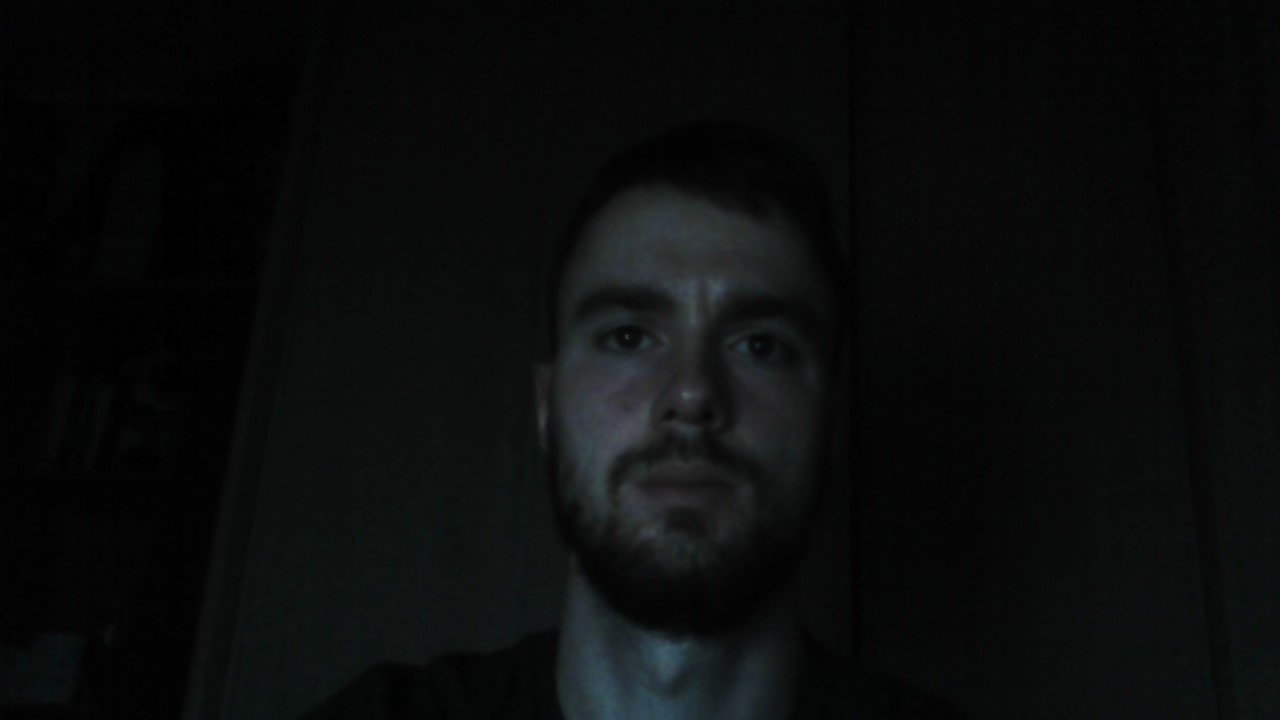
\includegraphics[width=\linewidth, height=20mm]{detekcja/12_input.jpg}
    	\end{minipage}
		& 
		\begin{minipage}{.2\textwidth}
      	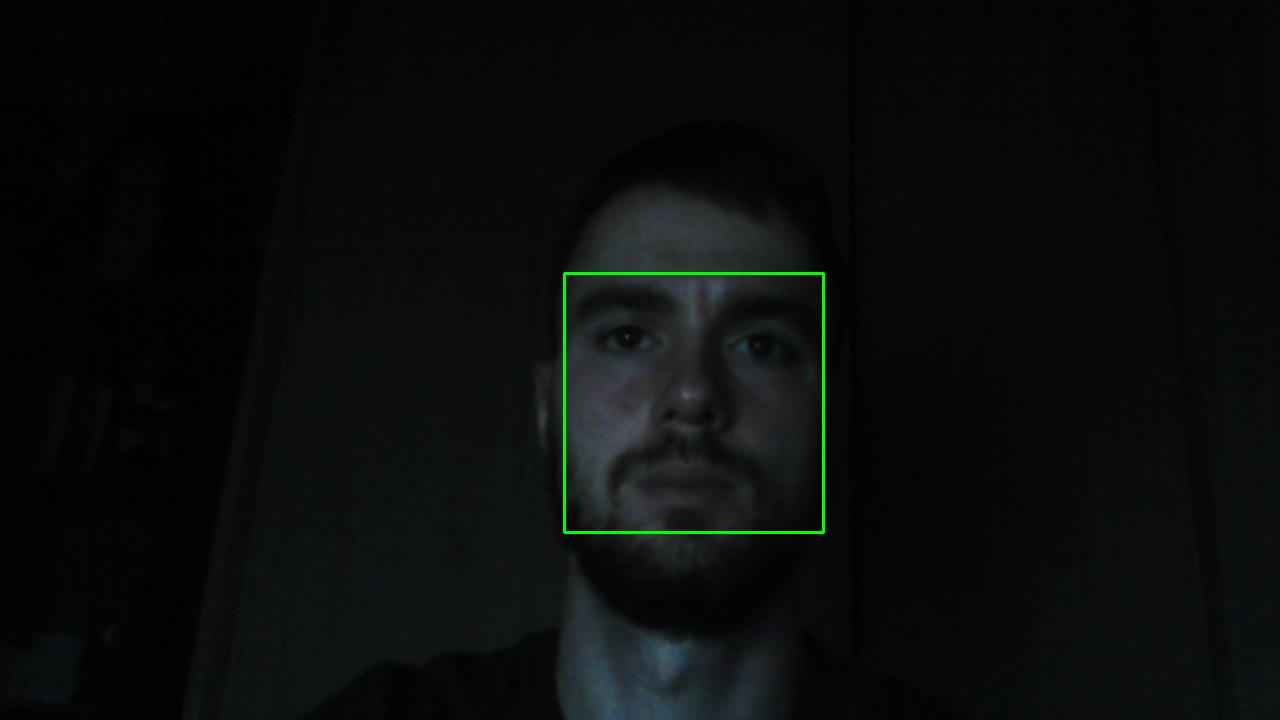
\includegraphics[width=\linewidth, height=20mm]{detekcja/12_haar.jpg}
    	\end{minipage}
		& 
		\begin{minipage}{.2\textwidth}
      	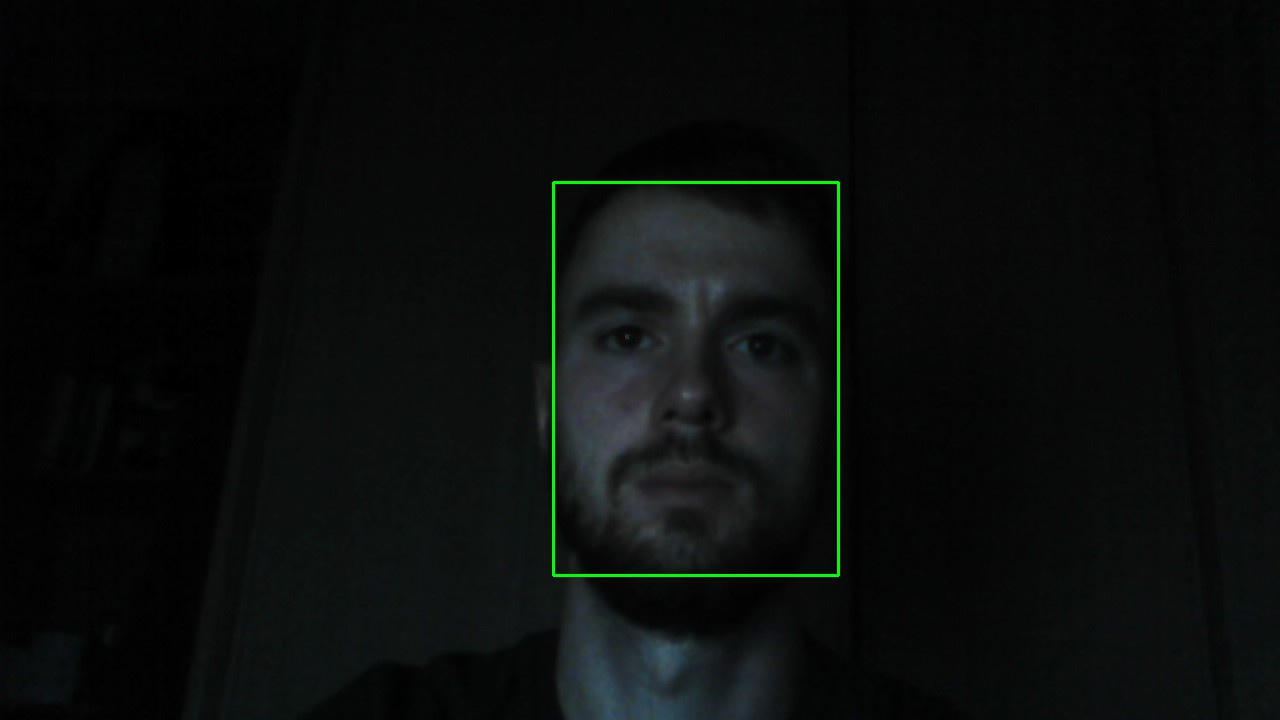
\includegraphics[width=\linewidth, height=20mm]{detekcja/12_dnn.jpg}
    	\end{minipage}
		& 
		\begin{minipage}{.2\textwidth}
      	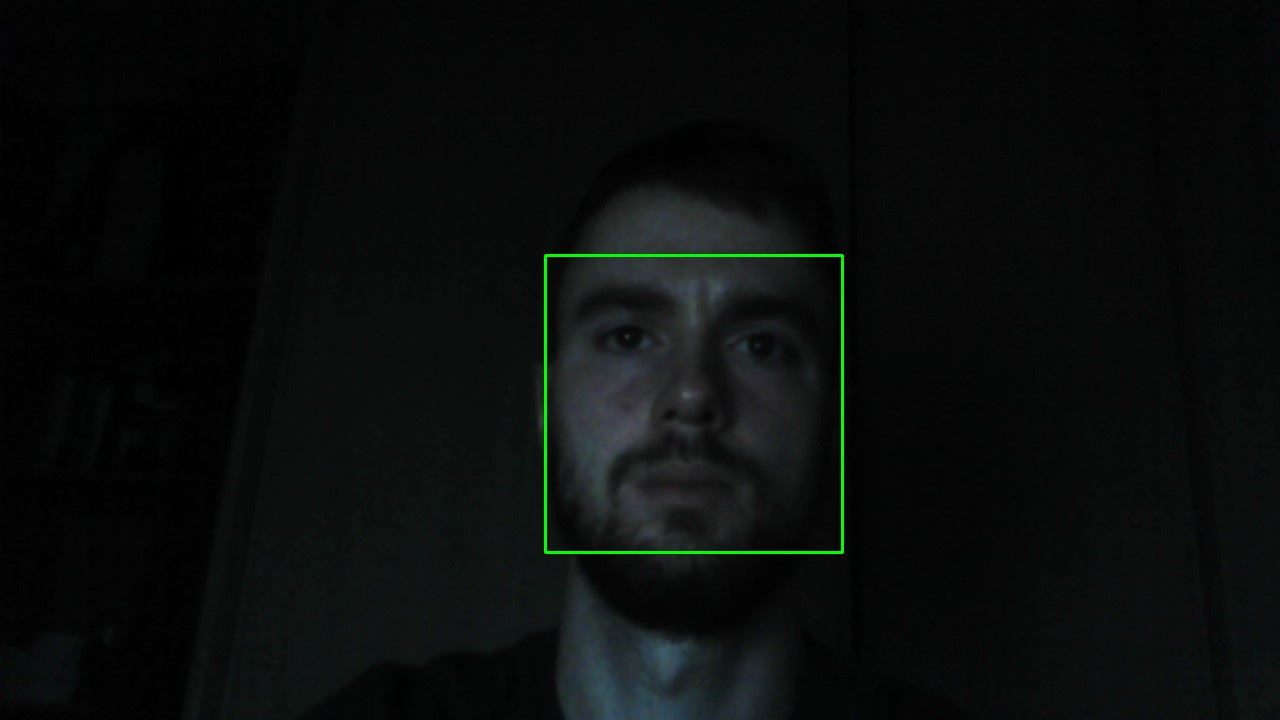
\includegraphics[width=\linewidth, height=20mm]{detekcja/12_azure.jpg}
    	\end{minipage}	
    	\\
  		\hline 
\caption{Porównanie działania detektorów w wybranych warunkach}
\label{tab:porownanie_detektorow}
\end{longtable}
Pierwszą różnicą, którą można zaobserwować w sposobie działania detektorów jest rozmiar obszaru twarzy oznaczany przez algorytmy. Najmniejszym z nich jest twarz wykrywana metodą Haara, oznaczany obszar zaczyna się na wysokości brwi i kończy niewiele poniżej ust. W przypadku detekcji twarzy z wykorzystaniem głębokiej sieci neuronowej prostokąt obejmuje także całe czoło oraz podbródek przedstawionej osoby. Rozmiar obszaru uzyskanego przez ACS(Azure Cognitive Services) mieści się pomiędzy metodą Haara a DNN(Deep Neural Network), obejmuję częściowo czoło i podbródek.

Każda z metod dobrze poradziła sobie w przypadku centralnego zdjęcia twarzy przy dobrym jak i słabym oświetleniu. Najskuteczniejszą z metod okazała się metoda DNN, która wykryła twarz na każdym z dziewięciu zdjęć. Metoda wykorzystująca platformę Azure okazała się nieskuteczna w przypadku zdjęcia przedstawiającego częściowo zakrytą twarz oraz z odchyloną głową. 

Najwrażliwszym na jakoś zdjęcia okazała się metoda Haara, która nie była w stanie sobie poradzić choćby z najmniejszymi zmianami w układzie twarzy na zdjęciu. Używając tego detektora nie udało się wykryć twarzy na obrazach, które nie sprawiły problemu pozostałym metodą. Między innymi nie wykryto twarzy na obrazie przedstawiającym profil oraz głowę przechyloną na bok.

Zbadano, że wysoka skuteczność detekcji twarzy metodą DNN wiąże się z większą ilością fałszywych detekcji w porównaniu z pozostałymi metodami. Z tego powodu wyniki uzyskane tą metodą należy filtrować,a jest to możliwe poprzez ustawienie pewności powyżej, której algorytm ma zwracać odpowiedzi.

Średnie czasy odpowiedzi detektorów przedstawiono w tabeli \ref{tab:systemy}. W najkrótszym czasie uzyskano odpowiedź od sieci neuronowej, a najwolniejsza zgodnie z oczekiwania była metoda wykorzystująca ACS. Znacznie dłuższy czas trwania wynika z konieczności skontaktowania się z serwerem z innego kraju.

\begin{table}[H]\label{tab:systemy}
	\centering
	\caption{Średni czas przetwarzania zadania detekcji twarzy}
	\scalebox{1.0}{
	\begin{tabular}{|c|c|c|c|}
  		\hline 
  		 & \bfseries Haar & \bfseries Dnn & \bfseries ACS\\
  		\hline
  		\bfseries Średni czas odpowiedzi [s]& 0,023127109 &0,018201053 &0,465438843 \\
  		\hline
  	\end{tabular}
  	}
\end{table}

W celu potwierdzenia uzyskanych wniosków przeprowadzono końcowy test polegający na uruchomieniu każdego z detektorów na bazie profili składającej się z 2000 zdjęć. Wyniki przedstawiono na rysunku \ref{fig:porownanie_detektorow}. Detektor oparty o głęboką siec neuronową wykrył twarz na 94,6\% zdjęć, Azure 90,1\%, a Haar 88,7\%. Wyniki potwierdziły, że sieć neuronowa, w tym przypadku daje najlepsze rezultaty, korzystniejsze o nawet 6\% od pozostałych metod.

\begin{figure}[H]
	\centering
	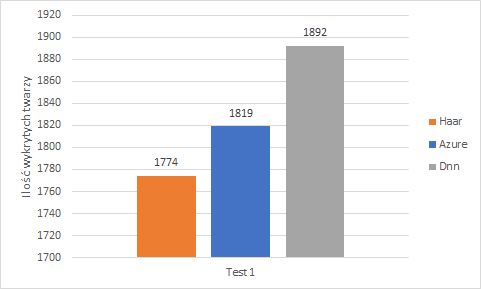
\includegraphics[scale=1.0]{porownanie_detektorow.png}
	\caption{Porównanie działania detektorów na bazie 2000 zdjęć}
	\label{fig:porownanie_detektorow}
\end{figure}

\section{Dane treningowe}
Za dane wejściowe do procesu trenowania sieci neuronowych wybrano \fnurl{Glasgow Unfamiliar Face Database (GUFD)}{http://www.facevar.com/glasgow-unfamiliar-face-database}, która dostępna jest za darmo i można jej używać na potrzeby badań uczelnianych oraz publikacji. Jedynym warunkiem użycia jest zacytowanie jednej z publikacji właściciela bazy.

Baza zawiera 303 tożsamości. Na każdą z tożsamości składa się 20 zdjęć jednej osoby wykonanych w różnych warunkach np. różniące się kąty ujęcia, wyrazy twarzy oraz z dodatkowymi akcesoriami(okulary, kaptur, czapka). 

Do materiałów uczących dodatkowo dodano profil autora tej pracy magisterskiej.

\section{Trenowanie sieci neuronowych}
Podczas badania sieci neuronowych postanowiono sprawdzić kilka podstawowych czynników, na które składa się wpływ ilości wybranych tożsamości oraz wpływ ilości zdjęć przydzielonych tożsamości na:
\begin{itemize}
\item czas potrzebny na preprocessing danych uczących,
\item czas trwania trenowania modelu,
\item rozmiar pliku zawierającego model (jeśli istnieje).
\end{itemize}
W rozdziale \ref{b:rozpoznawanie} omówiono wpływ wyżej wymienionych parametrów na czas oraz pewność identyfikowania tożsamości.

\subsection{Wpływ wybranych parametrów na przygotowanie danych uczących}
Zgodnie z oczekiwaniami, preprocessing danych wymagany przed trenowaniem identyfikatorów powiązanych z biblioteką OpenCv jest znacznie szybszy od Azure. Największą wadą wynikającą z chmurowości  ACS(Azure Cognitive Services) jest konieczność wykonania tysięcy zapytań, w tym większość z nich odpowiadających za przekazanie zdjęć do chmury. Prędkość dodawania danych jest ograniczana przez jakość połączenia z serwerem. Na przygotowanie 19 zdjęć dla 100 profili, system potrzebował około 15 minut, które może się wydawać astronomiczne w porównaniu z 24 sekundami potrzebnymi na przygotowanie danych dla metod trenowanych lokalnie.

Na rysunku \ref{fig:czas_p_profile} można zaobserwować że czas potrzebny na przygotowanie danych w przypadku OpenCv rósł liniowo. Podobny efekt był oczekiwany dla ACS. Brak liniowości może wynikać z różnych rozmiarów plików oraz chwilowej lepszej/gorszej jakości połączenia z serwerem.
\begin{figure}[H]
	\centering
	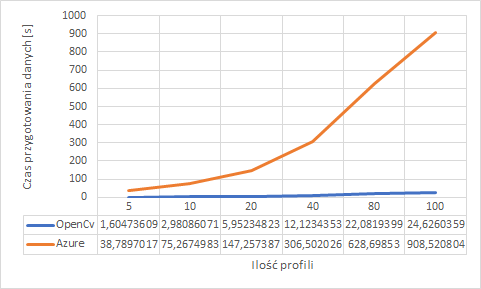
\includegraphics[scale=1.0]{czas_przygotowania_a_ilosc_profili.png}
	\caption{Wpływ ilości profili użytych podczas treningu na czas przygotowania danych uczących}
	\label{fig:czas_p_profile}
\end{figure}
Wyniki uzyskane podczas drugiego testu, które przedstawiono na grafie \ref{fig:czas_p_zdjecia} potwierdzają tezę o niestabilności połączenia z serwisem chmurowym. Dla tego testu udało się uzyskać zależność ilości zdjęć od czasu zbliżoną do liniowej.
\begin{figure}[H]
	\centering
	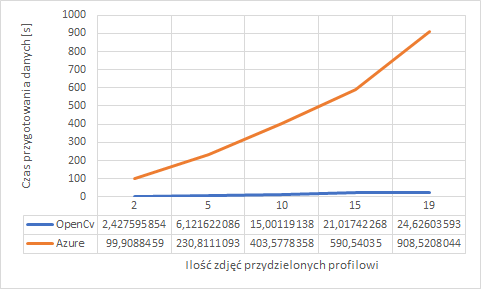
\includegraphics[scale=1.0]{czas_przygotowania_a_ilosc_zdjec.png}
	\caption{Wpływ ilości zdjęć przydzielonych profilowi na czas przygotowania danych uczących}
	\label{fig:czas_p_zdjecia}
\end{figure}

\subsection{Wpływ wybranych parametrów na czas trwania treningu}
Kolejnym interesującym testem, który przeprowadzona było zbadanie wpływu ilości użytych profili oraz ilości zdjęć przypisanych profilowi na czas trwania nauki. Zgodnie z oczekiwaniami wraz z przyrostem danych zwiększał się czas wymagany na wytrenowanie sieci. Wyniki przedstawiono na rysunku \ref{fig:czas_t_profile}. Wyjątkiem pozostało rozwiązanie chmurowe Azure, które niezależnie od ilości danych zawsze trwało sekundę (najmniejsza jednostka czasu, którą można uzyskać od usługi). Podobnym zachowaniem wykazał się algorytm LBPH (\ref{lbph}), w przypadku którego czas treningu wydłuż się od 0,7s do maksymalnie 12s. W przypadku pozostałych metod czas treningu wzrósł z początkowej wartości maksymalnie kilku sekund do nawet kilku minut
\begin{figure}[H]
	\centering
	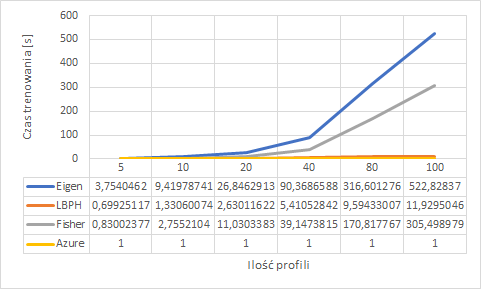
\includegraphics[scale=1.0]{czas_trenowania_a_ilosc_profili.png}
	\caption{Wpływ ilości profili użytych podczas treningu na czas trenowania sieci}
	\label{fig:czas_t_profile}
\end{figure}
Bliźniaczy test przeprowadzony dla zmiennej ilości zdjęć przypisanej do profilu zakończył się wynikami zbliżonymi do poprzedniego badania. Przyrost czasu pozostał nieliniowy.
\begin{figure}[H]
	\centering
	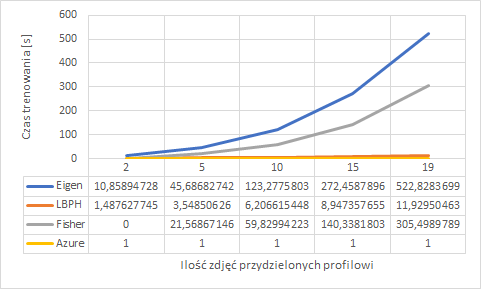
\includegraphics[scale=1.0]{czas_trenowania_a_ilosc_zdjec.png}
	\caption{Wpływ ilości zdjęć przydzielonych profilowi na czas trenowania sieci}
	\label{fig:czas_t_zdjecia}
\end{figure}

\subsection{Wpływ wybranych parametrów na rozmiar modelu sieci}
Wyniki uzyskane podczas badaniu wpływu parametrów na rozmiar utworzonego modelu przedstawiono na rysunku \ref{fig:rozmiar_profile} oraz \ref{fig:rozmiar_zdjecia}. Ze względu na brak dostępu do informacji o rozmiarze modelu, Azure Cognitve Services został pominięty podczas tego testu.

W badaniu z poprzedniego rozdziału okazało się, że proces trenowania algorytmu Eigen jest najbardziej czasochłonny. Ta informacja ma swoje odzwierciedlenie w rozmiarze modelu. Rozmiar modelu uzyskany dla maksymalnej ilości wykorzystanych profili osiągnął wartość aż 3GB, które w porównaniu do 163MB dla LBPH oraz 197MB dla metody Fishera jest ogromną wartością. W uproszczeniu można by powiedzieć że wzrost rozmiaru pliku był liniowy i zwiększał się dwukrotnie wraz z dwukrotnym zwiększeniem się ilości wykorzystanych profili. 
\begin{figure}[H]
	\centering
	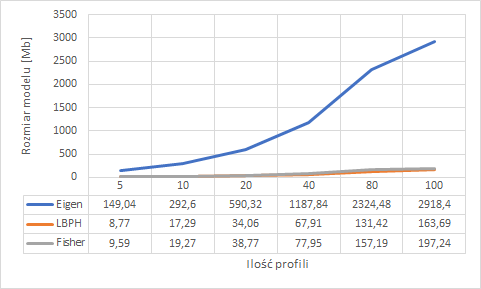
\includegraphics[scale=1.0]{rozmiar_modelu_a_ilosc_profili.png}
	\caption{Wpływ ilości profili użytych podczas treningu na rozmiar utworzonego modelu}
	\label{fig:rozmiar_profile}
\end{figure}
W przypadku badania wpływu ilości zdjęć przypisanych do profilu na rozmiar pliku, wystąpił problem z uzyskaniem pierwszej próbki dla metody Fishera, która jak się okazało wymaga minimalnie 3 zdjęć przypisanych do profilu. Podobnie jak w poprzednim teście algorytm Eigen oraz LBPH zachowywał się liniowo co jest dobrze widoczne na rysunku \ref{fig:rozmiar_zdjecia}. Interesującym zachowaniem wykazał się model utworzony dla metody Fishera, który już przy 5 zdjęciach osiągnął wartość minimalnie różniącą się od maksymalnej. Dodawanie kolejnych zdjęć każdemu z profili powodowało minimalne zmiany w rozmiarze pliku. Uzyskane zachowanie znacznie różniło się od wyników z testu poprzedniego (rysunek \ref{fig:rozmiar_profile}).
\begin{figure}[H]
	\centering
	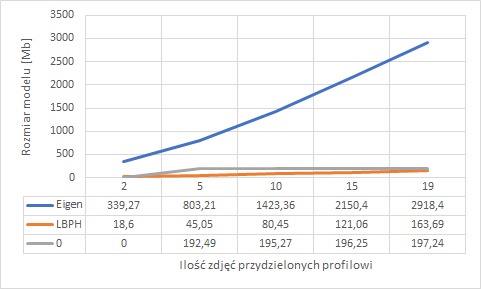
\includegraphics[scale=1.0]{rozmiar_modelu_a_ilosc_zdjec.png}
	\caption{Wpływ ilości zdjęć przydzielonych profilowi na rozmiar utworzonego modelu}
	\label{fig:rozmiar_zdjecia}
\end{figure}

\section{Rozpoznawanie twarzy} \label{b:rozpoznawanie}
Kolejnym etapem badań było przetestowanie działania identyfikatorów twarzy, Testy podzielono na 3 kategorie:
\begin{itemize}
\item wpływ ilości zdjęc przypisanych do profilu na pewność rozpoznania
\item wpływ ilości profili użytych podczas treningu na pewność rozpoznania
\item test wszystkich próbek
\end{itemize}
\subsection{Wpływ ilości zdjęć przypisanych do profilu na pewność rozpoznania}
Metody dostępne w bibliotece OpenCv różnią się od Azure sposobem określania pewności identyfikacji. ACS (Azure Cognitive Services) zwraca pewność w postaci procentowej, a OpenCv jako wektor oddalenia od najbliższej próbki, którego im wartość jest mniejsza tym lepiej.

W pierwszym etapie wykorzystano sieci nauczone podczas badań z rozdziału poprzedniego do identyfikacji jednego ze zdjęć. Wybrane zdjęcie zostało poprawnie zidentyfikowane przez każdą z metod.
\begin{figure}[H]
	\centering
	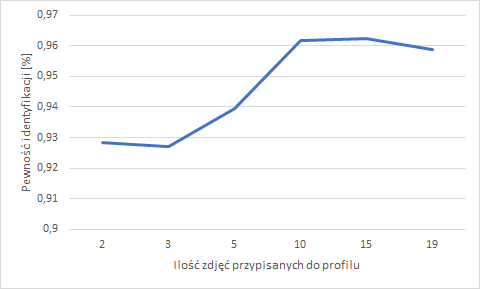
\includegraphics[scale=1.0]{azure_pewnosc_a_ilosc_zdjec.png}
	\caption{Wpływ ilości zdjęć przydzielonych profilowi na pewność identyfikacji Azure. Użyto 100 profili}
	\label{fig:azure_zdjecia}
\end{figure}
\begin{figure}[H]
	\centering
	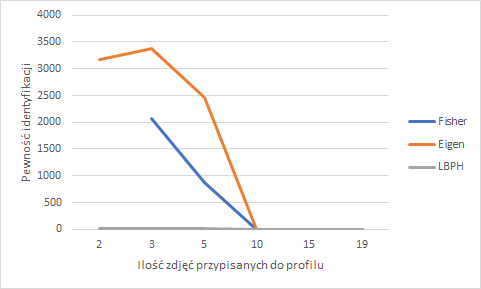
\includegraphics[scale=1.0]{opencv_pewnosc_a_ilosc_zdjec.png}
	\caption{Wpływ ilości zdjęć przydzielonych profilowi na pewność identyfikacji OpenCv. Użyto 100 profili}
	\label{fig:opencv_zdjecia}
\end{figure}

\subsection{Wpływ ilości profili użytych podczas treningu na pewność rozpoznania}
Przy 19 zdjeciach na profil, twarzy identyfikowane były bardzo dobrze i nie bylo widac roznicy w pewnosci identyfikacji.
\begin{figure}[H]
	\centering
	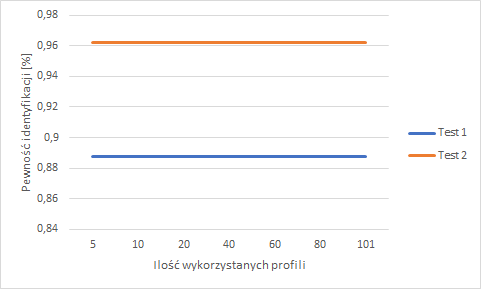
\includegraphics[scale=1.0]{10_azure_pewnosc_a_ilosc_profili.png}
	\caption{Wpływ ilości profili użytych podczas nauki na pewność identyfikacji Azure. Użyto 10 zdjęć dla każdego profilu}
	\label{fig:azure_10__profile}
\end{figure}
Przy 10 zdjęciach nie bylo roznicy dla metod OpenCv
\begin{figure}[H]
	\centering
	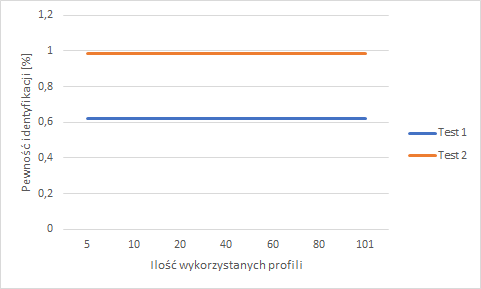
\includegraphics[scale=1.0]{5_azure_pewnosc_a_ilosc_profili.png}
	\caption{Wpływ ilości profili użytych podczas nauki na pewność identyfikacji Azure. Użyto 5 zdjęć dla każdego profilu}
	\label{fig:azure_5__profile}
\end{figure}
\begin{figure}[H]
	\centering
	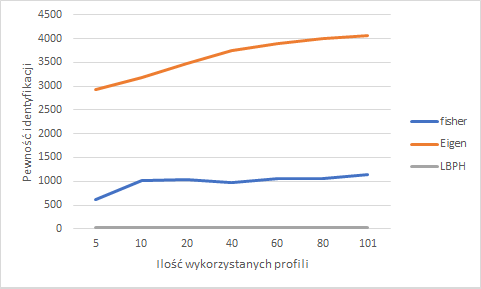
\includegraphics[scale=1.0]{5_opencv_pewnosc_a_ilosc_profili.png}
	\caption{Wpływ ilości profili użytych podczas nauki na pewność identyfikacji OpenCv. Użyto 5 zdjęć dla każdego profilu}
	\label{fig:azure_5__profile}
\end{figure}

\subsection{Porównanie wyników}
\begin{figure}[H]
	\centering
	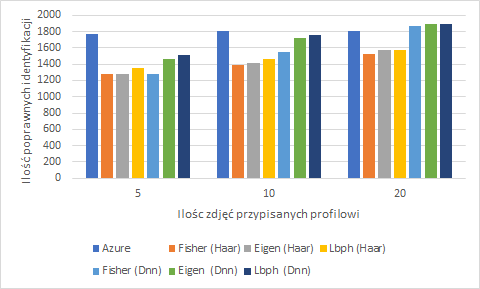
\includegraphics[scale=1.0]{porownanie_identyfikacji.png}
	\caption{Porównanie działania usług rozpoznających na bazie 2000 zdjęć}
	\label{fig:porownanie_identyfikator}
\end{figure}


\subsection{Czas przetwarzania zapytania}

\section{Ocena przydatności wybranych usług IoT}



Konfiguracja bazy danych oraz maszyny wirtualnej okazała się równie prosta w każdym ze środowisk. Proces konfiguracji odbywał się poprzez wypełnienie kilku formularzy niewymagających wprowadzania dużej ilości informacji (ze względu na ograniczenia studenckiej licencji). Na końcu procesu uzyskany zostaje connection string oraz konto za pomocą, którego można zalogować się na serwer.

Największa różnica między dwoma dostawcami wystąpiła w przypadku usług hostujących aplikację webową czyli Azure App Service oraz AWS Elastic Beanstalk. Podczas pierwszych testów konfiguracji aplikacja internetowa istniała jedynie w rozwiązaniu przygotowanym w języku Angular 4. Struktura aplikacji została przygotowana na podstawie wzoru przygotowanego przez Microsoft. Azure App Service bezproblemowo wspierał nawet najnowsze wersje rozwiązań przygotowanych dla .NET Core 2. Niestety AWS nie był przygotowany 